% % Preamble BEGINN %%%%%%%%%%%%%%%%%%%%%%%%%%%%%%%%%%%%%%%%%%%%%%%%%%%%%%%%%

%%% Preamble (Dokumentenklasse)
% ------------------------------------------------------------------------
% LaTeX - Preambel ******************************************************
% ------------------------------------------------------------------------
% Dokumentklasse (Koma Script)
% ------------------------------------------------------------------------
% basiernd auf www.matthiaspospiech.de/latex/vorlagen Diplomarbeit kompakt
% ========================================================================
\documentclass[%
   %draft,            % Entwurfsstadium
   final,             % fertiges Dokument
   12pt,              % Schriftgroesse der Grundschrift
   bigheadings,       % gro�e �berschriften
   ngerman,           % wird an andere Pakete weitergereicht
   a4paper,           % Papierformat
   BCOR5mm,          % Bindekorrektur: Zus�tzlicher Rand auf der Innenseite
   DIV14,            % Seitengr��e (siehe Koma Skript Dokumentation !)
   1.1headlines,     % Zeilenanzahl der Kopfzeilen
   pagesize,         % Schreibt die Papiergroesse in die Datei.
   oneside,          % Einseitiges Layout
%   twoside,          % Zweiseitiges Layout
   openright,        % Kapitel beginnen immer auf der rechten Seite
   titlepage,        % Titel als einzelne Seite ('titlepage' Umgebung)  
   headsepline,      % Linie unter Kolumnentitel ()
%   plainheadsepline, % Linie unter Kolumnentitel () plain Seitenstil
   nochapterprefix,  % keine Ausgabe von 'Kapitel:'
   bibtotoc,         % Bibliographie ins TOC
%	bibtotocnumbered, % Bibliographie ins TOC mit Kapitelnummer
   tocindent,        % eingereuckte Gliederung
   listsindent,      % eingereuckte LOT, LOF
   pointlessnumbers, % �berschriftnummerierung ohne Punkt, siehe DUDEN !
   cleardoubleempty, % Leere linke Seite bei Zweiseitenlayout vor Kapitel
   fleqn,            % Formeln werden linksbuendig angezeigt
%   parindent,        % Absatz mit Einzug (Standard)
   halfparskip,      % Absatz halbe Zeile Abstand
%   parskip,          % Absatz ganze Zeile Abstand
]{scrbook}%     Klassen: scrartcl, scrreprt, scrbook


%%% Alle Namen usw. im Titel und im hyperref-Paket
% ------------------------------------------------------------------------
% LaTeX - Preambel ******************************************************
% ------------------------------------------------------------------------
% pre-work
% ========================================================================
% % ToDo kennzeichnen
\newcommand{\workTodo}[1]{\textcolor{red}{todo: #1}}

% % F�r Datum und Zeit in Fusszeile
% % !!!Inhalt bei Fertigstellung der Arbeit l�schen
\newcommand{\workMarkDateTime}{\today{}  }

% % Alle Namen werden im Titel und im hyperref-Paket eingetragen
% % !!! Ueberall f�r <Wert> das Entsprechende eintragen

 % <Typ> Studienarbeit, Dipolmarbeit, Studienarbeit oder Bachlor-Abschlussarbeit
\newcommand{\workTyp}{Team Project\xspace}

 % <Titel> der Arbeit
\newcommand{\workTitel}{Quadrocopter}

 % <Studiengang> z.B. Kommunikationstechnik
\newcommand{\workStudiengang}{ASM-SB \xspace}

% <Semester> mit Jahr z.B. Sommersemester 2008  
\newcommand{\workSemester}{ASM2\xspace}

% <Name> des Studenten
\newcommand{\workNameStudentOne}{Oliver Breuning\xspace}
\newcommand{\workNameStudentTwo}{Martin Brodbeck\xspace}
\newcommand{\workNameStudentThree}{J\"urgen Schmidt\xspace}
\newcommand{\workNameStudentFour}{Phillip Woditsch\xspace}

% <Pruefer> Name des pr�fenden (betreuenden) Professor an der Hochschule
\newcommand{\workPruefer}{Prof. Dr. J\"org Friedrich\xspace} 


% %%% Nur bei Abschluss-Arbeiten

% <Datum> der Abgabe der Arbeit (Eidesstatliche Erkl�rung)
\newcommand{\workDatum}{\today\xspace}

% <Zweitpr�fer>
\newcommand{\workZweitPruefer}{\workTodo{<Zweitpr�fer>}\xspace}

% <Zeitraum>
\newcommand{\workZeitraum}{Summersemester 2015\xspace}


% %%% Nur bei Industrie-Arbeiten:

% <Firma>
\newcommand{\workFirma}{\workTodo{<Firma>}\xspace}

% <Betreuer in der Firma>
\newcommand{\workBetreuer}{\workTodo{<Betreuer in der Firma>}\xspace}

% Firmenlogo Name hier anpassen, Gr��e (wenn m�glich) nicht �ndern
%\newcommand{\workFirmenLogo}{
\includegraphics[width=5cm]{fig/aa-titel/Bosch_4C_S}} 


%%% Preamble (Pakete)
% ------------------------------------------------------------------------
% LaTeX - Preambel ******************************************************
% ------------------------------------------------------------------------
% Packages
% ------------------------------------------------------------------------
% basiernd auf www.matthiaspospiech.de/latex/vorlagen Diplomarbeit kompakt
% ========================================================================

% Inhalt:
% 1. Einige Pakete muessen unbedingt vor allen anderen geladen werden
% 2. Fonts Fonts Fonts
% 3. Math Packages
% 4. Symbole
% 5. text related packages
% 6. Pakete zum Zitieren
% 7. PDF related packages
% 8. Tables (Tabular)
% 9. figures and placement
% 10. verbatim packages
% 11. science packages
% 12. layout packages

% ~~~~~~~~~~~~~~~~~~~~~~~~~~~~~~~~~~~~~~~~~~~~~~~~~~~~~~~~~~~~~~~~~~~~~~~~
% Encoding der Dateien (sonst funktionieren Umlaute nicht)
% Empfohlen latin1, da einige Pakete mit utf8 Zeichen nicht
% funktionieren, z.B: listings, soul.

\usepackage[latin1]{inputenx} % ISO-8859-1
%\usepackage[ansinew]{inputenx} % Windows-Standard (CP1252) (baut auf ISO 8859-1 und ISO 8859-15 auf)
%\usepackage[utf8]{inputenc}

% ~~~~~~~~~~~~~~~~~~~~~~~~~~~~~~~~~~~~~~~~~~~~~~~~~~~~~~~~~~~~~~~~~~~~~~~~
% 1. Einige Pakete muessen unbedingt vor allen anderen geladen werden
% ~~~~~~~~~~~~~~~~~~~~~~~~~~~~~~~~~~~~~~~~~~~~~~~~~~~~~~~~~~~~~~~~~~~~~~~~
%
\usepackage{xspace} % Define commands that don't eat spaces.
\usepackage{ifpdf} % Fuer Pakete/Paketoptionen, die nur fuer pdf benoetigt werden \ifpdf \else \fi
\usepackage{calc} % Calculation with LaTeX
\usepackage[english]{babel} % Languagesetting
\usepackage[table]{xcolor} % Farben
\usepackage[]{graphicx} % Bilder
%\usepackage{epstopdf} % If an eps image is detected, epstopdf is automatically called to convert it to pdf format.
\usepackage[]{amsmath} % Amsmath - Mathematik Basispaket
\usepackage{ragged2e} % Besserer Flatternsatz (Linksbuendig, statt Blocksatz)

% ~~~~~~~~~~~~~~~~~~~~~~~~~~~~~~~~~~~~~~~~~~~~~~~~~~~~~~~~~~~~~~~~~~~~~~~~
% 2. Fonts Fonts Fonts
% ~~~~~~~~~~~~~~~~~~~~~~~~~~~~~~~~~~~~~~~~~~~~~~~~~~~~~~~~~~~~~~~~~~~~~~~~

\usepackage[T1]{fontenc} % T1 Schrift Encoding (notwendig f�r die meisten Type 1 Schriften)
\usepackage{textcomp}	 % Zusatzliche Symbole (Text Companion font extension)

% Alle Schriften die hier angegeben sind sehen im PDF richtig aus.
% Die LaTeX Standardschrift ist die Latin Modern (lmodern Paket).
% If Latin Modern is not available for your distribution you must install the
% package cm-super instead. Otherwise your fonts will look horrible in the PDF

% DO NOT LOAD ae-Package for the font !

%% - Latin Modern
\usepackage{lmodern}
%% -------------------
%
% % - Times, Helvetica, Courier (Word Standard...)
%\usepackage{mathptmx}
%\usepackage[scaled=.90]{helvet}
%\usepackage{courier}
% % -------------------
%%
%% - Palantino , Helvetica, Courier
%\usepackage{mathpazo}
%\usepackage[scaled=.95]{helvet}
%\usepackage{courier}
%% -------------------
%
%% - Bera Schriften
%\usepackage{bera}
%% -------------------
%
%% - Charter, Bera Sans
%\usepackage{charter}\linespread{1.05}
%\renewcommand{\sfdefault}{fvs}


% ~~~~~~~~~~~~~~~~~~~~~~~~~~~~~~~~~~~~~~~~~~~~~~~~~~~~~~~~~~~~~~~~~~~~~~~~
% 3. Math Packages
% ~~~~~~~~~~~~~~~~~~~~~~~~~~~~~~~~~~~~~~~~~~~~~~~~~~~~~~~~~~~~~~~~~~~~~~~~

\usepackage[fixamsmath,disallowspaces]{mathtools} % Erweitert amsmath und behebt einige Bugs
\usepackage{fixmath}
\usepackage[all,warning]{onlyamsmath} % Warnt bei Benutzung von Befehlen die mit amsmath inkompatibel sind.
\usepackage{icomma} % Erlaubt die Benutzung von Kommas im Mathematikmodus

% ~~~~~~~~~~~~~~~~~~~~~~~~~~~~~~~~~~~~~~~~~~~~~~~~~~~~~~~~~~~~~~~~~~~~~~~~
% 4. Symbole
% ~~~~~~~~~~~~~~~~~~~~~~~~~~~~~~~~~~~~~~~~~~~~~~~~~~~~~~~~~~~~~~~~~~~~~~~~
\usepackage{amssymb}
%\usepackage{wasysym}
%\usepackage{marvosym}
%\usepackage{pifont}

% ~~~~~~~~~~~~~~~~~~~~~~~~~~~~~~~~~~~~~~~~~~~~~~~~~~~~~~~~~~~~~~~~~~~~~~~~
% 5. text related packages
% ~~~~~~~~~~~~~~~~~~~~~~~~~~~~~~~~~~~~~~~~~~~~~~~~~~~~~~~~~~~~~~~~~~~~~~~~

\usepackage{url} % Setzen von URLs. In Verbindung mit hyperref sind diese auch aktive Links.
\usepackage[stable,perpage, ragged,  multiple]{footmisc} % Fussnoten
\usepackage[ngerman]{varioref} % Intelligente Querverweise
\usepackage{enumitem} % Listen

% ~~~~~~~~~~~~~~~~~~~~~~~~~~~~~~~~~~~~~~~~~~~~~~~~~~~~~~~~~~~~~~~~~~~~~~~~
% 6. Pakete zum Zitieren
% ~~~~~~~~~~~~~~~~~~~~~~~~~~~~~~~~~~~~~~~~~~~~~~~~~~~~~~~~~~~~~~~~~~~~~~~~

\usepackage[babel, german=quotes, english=british, french=guillemets]{csquotes} % clever quotations
\SetBlockThreshold{2} % Anzahl von Zeilen
\newenvironment{myquote}%
          {\begin{quote}\small}%
          {\end{quote}}%
\SetBlockEnvironment{myquote}

% ~~~~~~~~~~~~~~~~~~~~~~~~~~~~~~~~~~~~~~~~~~~~~~~~~~~~~~~~~~~~~~~~~~~~~~~~
% 7. PDF related packages
% ~~~~~~~~~~~~~~~~~~~~~~~~~~~~~~~~~~~~~~~~~~~~~~~~~~~~~~~~~~~~~~~~~~~~~~~~

\ifpdf % Wenn als PDF ausgegeben wird
\usepackage{pdfpages} % pdf-Seiten einbinden
\usepackage[pdftex]{hyperref} % PDF Option in Hyperref
\else
\usepackage[dvipdfm]{hyperref}
\fi

%%% Doc: ftp://tug.ctan.org/pub/tex-archive/macros/latex/contrib/pdfpages/pdfpages.pdf
%\usepackage{pdfpages} % Include pages from external PDF documents in LaTeX documents

%%% Doc: ftp://tug.ctan.org/pub/tex-archive/macros/latex/contrib/hyperref/doc/manual.pdf
\hypersetup{
          pdfhighlight = /O,	         % Visualisierung beim anklicken von Links
% Farben fuer die Links
   colorlinks=true,	        % Links erhalten Farben statt Kaestchen
   urlcolor=darkblue,    % \href{...}{...} external (URL)
   filecolor=darkblue,  % \href{...} local file
   linkcolor=darkblue,  % \ref{...} and \pageref{...}
          citecolor =darkblue,    % Literaturverzeichnis
   % Links
   raiselinks=true,			 % calculate real height of the link
   breaklinks,	        % Links bestehen bei Zeilenumbruch
%   backref=page,	         % Backlinks im Literaturverzeichnis (section, slide, page, none)
%   pagebackref=true,        % Backlinks im Literaturverzeichnis mit Seitenangabe
   verbose,
%   hyperindex=true,         % backlinkex index
   linktocpage=true,        % Inhaltsverzeichnis verlinkt Seiten
%   hyperfootnotes=false,	% Keine Links auf Fussnoten
   % Bookmarks
%   bookmarks=true,	         % Erzeugung von Bookmarks fuer PDF-Viewer
   bookmarksopenlevel=1,    % Gliederungstiefe der Bookmarks
   bookmarksopen=true,      % Expandierte Untermenues in Bookmarks
   bookmarksnumbered=true,  % Nummerierung der Bookmarks
   bookmarkstype=toc,       % Art der Verzeichnisses
   % Anchors
   plainpages=false,        % % Make page anchors using the formatted form of the page number. With this option, hyperref writes different anchors for pages �ii� and �2�. (If the option is set �true� � the default � hyperref writes page anchors as the arabic form of the absolute page number, rather than the formatted form.)
   % hypertexnames=false,
   pageanchor=true,	        % Pages are linkable
   % PDF Informationen
   pdftitle={\workTyp: \workTitel},	        % Titel
   pdfauthor={\workNameStudentOne},	    % Autor
   pdfcreator={LaTeX, hyperref, KOMA-Script}, % Ersteller
   %pdfproducer={pdfeTeX 1.10b-2.1} %Produzent
   pdfstartview=FitH,       % Dokument wird Fit Width geaefnet
   pdfpagemode=UseOutlines, % Bookmarks im Viewer anzeigen
%   pdfpagelabels=true,      % set PDF page labels
}

% ~~~~~~~~~~~~~~~~~~~~~~~~~~~~~~~~~~~~~~~~~~~~~~~~~~~~~~~~~~~~~~~~~~~~~~~~
% 8. Tables (Tabular)
% ~~~~~~~~~~~~~~~~~~~~~~~~~~~~~~~~~~~~~~~~~~~~~~~~~~~~~~~~~~~~~~~~~~~~~~~~

\usepackage{booktabs}
\usepackage{tabularx} % tabularx nach hyperref laden
\usepackage{multirow}

\usepackage{dirtree}

% ~~~~~~~~~~~~~~~~~~~~~~~~~~~~~~~~~~~~~~~~~~~~~~~~~~~~~~~~~~~~~~~~~~~~~~~~
% 9. figures and placement
% ~~~~~~~~~~~~~~~~~~~~~~~~~~~~~~~~~~~~~~~~~~~~~~~~~~~~~~~~~~~~~~~~~~~~~~~~

%% Bilder und Graphiken ==================================================

\usepackage{float}	% Stellt die Option [H] fuer Floats zur Verfgung
\usepackage{flafter} % Floats immer erst nach der Referenz setzen
\usepackage{subfig} % Layout wird weiter unten festgelegt !
\usepackage{wrapfig} % Bilder von Text Umfliessen lassen

\usepackage{placeins} % Alle Floats bis \FloatBarrier ausgeben

% Make float placement easier
\renewcommand{\floatpagefraction}{.75} % vorher: .5
\renewcommand{\textfraction}{.1}       % vorher: .2
\renewcommand{\topfraction}{.8}        % vorher: .7
\renewcommand{\bottomfraction}{.5}     % vorher: .3
\setcounter{topnumber}{3}	         % vorher: 2
\setcounter{bottomnumber}{2}	         % vorher: 1
\setcounter{totalnumber}{5}	         % vorher: 3


% ~~~~~~~~~~~~~~~~~~~~~~~~~~~~~~~~~~~~~~~~~~~~~~~~~~~~~~~~~~~~~~~~~~~~~~~~
% 10. verbatim packages
% ~~~~~~~~~~~~~~~~~~~~~~~~~~~~~~~~~~~~~~~~~~~~~~~~~~~~~~~~~~~~~~~~~~~~~~~~

%%% Doc: ftp://tug.ctan.org/pub/tex-archive/macros/latex/contrib/upquote/upquote.sty
\usepackage{upquote} % Setzt "richtige" Quotes in verbatim-Umgebung

%%% Doc: No Documentation
% \usepackage{verbatim} % Reimplemntation of the original verbatim

%%% Doc: http://www.cs.brown.edu/system/software/latex/doc/fancyvrb.pdf
% \usepackage{fancyvrb} % Superior Verbatim Class

%% Listings Paket ------------------------------------------------------
%%% Doc: ftp://tug.ctan.org/pub/tex-archive/macros/latex/contrib/listings/listings-1.3.pdf
\usepackage{listings}

\lstset{
basicstyle =\ttfamily\color{black}\small, % Standardschrift
keywordstyle =, % \bfseries\color{blue}	  % Schl�sselwort-Style
%identifierstyle =\underbar,
commentstyle =\color{teal},
stringstyle =\itshape,
numbers = left,			  % Ort der Zeilennummern
numberstyle =\tiny\color{black},	   % Stil der Zeilennummern
numbers = left,			  % Ort der Zeilennummern
tabsize=2,			  % Groesse von Tabs
breaklines,			  % Zeilen werden Umgebrochen
breakatwhitespace,			  % An Leerzeichen umbrechen
%showspaces=true,			  % Leerzeichen anzeigen
backgroundcolor=\color{lightgray},	  % % Hintergrundfarbe der Listings
}
 \lstloadlanguages{% Check Dokumentation for further languages ...
%	[Visual]Basic
         [AlLaTeX]TeX,
         %Pascal
         %C
         %C++
         %XML
         %HTML
 }

%%% Doc: ftp://tug.ctan.org/pub/tex-archive/macros/latex/contrib/examplep/eurotex_2005_examplep.pdf
% LaTeX Code und Ergebnis nebeneinander darstellen
%\usepackage{examplep}


% ~~~~~~~~~~~~~~~~~~~~~~~~~~~~~~~~~~~~~~~~~~~~~~~~~~~~~~~~~~~~~~~~~~~~~~~~
% 11. science packages
% ~~~~~~~~~~~~~~~~~~~~~~~~~~~~~~~~~~~~~~~~~~~~~~~~~~~~~~~~~~~~~~~~~~~~~~~~

\usepackage[squaren]{SIunits}

% ~~~~~~~~~~~~~~~~~~~~~~~~~~~~~~~~~~~~~~~~~~~~~~~~~~~~~~~~~~~~~~~~~~~~~~~~
% 12. layout packages
% ~~~~~~~~~~~~~~~~~~~~~~~~~~~~~~~~~~~~~~~~~~~~~~~~~~~~~~~~~~~~~~~~~~~~~~~~

%% Zeilenabstand =========================================================
%
%%% Doc: ftp://tug.ctan.org/pub/tex-archive/macros/latex/contrib/setspace/setspace.sty
\usepackage{setspace}
%\doublespace	        % 2-facher Abstand
%\onehalfspace	  % 1,5-facher Abstand
% hereafter load 'typearea' again

%% Seitenlayout ==========================================================
%
% Layout mit 'typearea'
\typearea[current]{last}
\raggedbottom     % Variable Seitenhoehen zulassen


%% Kopf und Fusszeilen====================================================
%%% Doc: ftp://tug.ctan.org/pub/tex-archive/macros/latex/contrib/koma-script/scrguide.pdf
\usepackage[%
   automark,	 % automatische Aktualisierung der Kolumnentitel
   nouppercase,	 % Grossbuchstaben verhindern
]{scrpage2}

\usepackage{scrtime} % Zeit
%\usepackage{scrdate} % Datum

\pagestyle{scrheadings} % Seite mit Headern
%\pagestyle{scrplain} % Seiten ohne Header
%\pagestyle{empty} % Seiten ohne Header

% loescht voreingestellte Stile
\clearscrheadings
\clearscrplain
%
% [scrplain]{scrheadings}

% %%% Kopfzeile
% einseitig: Bei einseitigem Layout, nur folgende Zeilen verwenden !!!
\ihead[]{\leftmark} % links: Kapitel
 %\chead[\pagemark]{\pagemark} % mitte:
\ohead[]{\rightmark} % rechts: Section

% %zweiseitig: Bei zweiseitigem Layout, nur folgende Zeilen verwenden !!!
%\ihead[]{} % innen
% % \chead[\pagemark]{\pagemark} % mitte:
%\ohead[]{\headmark} % aussen: Kapitel (linke Seite) und Section (rechte Seite)
%
% %%% Fusszeile
\ifoot[\workMarkDateTime]{\workMarkDateTime} % innen:
%\cfoot[\pagemark]{\pagemark} % mitte:
\ofoot[\pagemark]{\pagemark} % aussen: Seitenzahl

% Angezeigte Abschnitte im Header
\automark[section]{chapter} % Inhalt von [\rightmark]{\leftmark}
%
% Linie zwischen Kopf und Textk�rper
\setheadsepline{.4pt}[\color{black}]

%% Fussnoten =============================================================
% Keine hochgestellten Ziffern in der Fussnote (KOMA-Script-spezifisch):
\deffootnote{1.5em}{1em}{\makebox[1.5em][l]{\thefootnotemark}}
\addtolength{\skip\footins}{\baselineskip} % Abstand Text <-> Fussnote
\setlength{\dimen\footins}{10\baselineskip} % Beschraenkt den Platz von Fussnoten auf 10 Zeilen
\interfootnotelinepenalty=10000 % Verhindert das Fortsetzen von
                                % Fussnoten auf der gegen�berligenden Seite

%% Schriften (Sections )==================================================

% -- Koma Schriften --
\newcommand\SectionFontStyle{\sffamily}

\setkomafont{chapter}{\huge\SectionFontStyle}    % Chapter
\setkomafont{sectioning}{\SectionFontStyle} %  % Titelzeilen % \bfseries

\setkomafont{pagenumber}{\bfseries\SectionFontStyle} % Seitenzahl
\setkomafont{pagehead}{\small\sffamily}	       % Kopfzeile

\setkomafont{descriptionlabel}{\itshape}        % Stichwortliste
%
\renewcommand*{\raggedsection}{\raggedright} % Titelzeile linksbuendig, haengend
%

%% Captions (Schrift, Aussehen) ==========================================

%%% Doc: ftp://tug.ctan.org/pub/tex-archive/macros/latex/contrib/caption/caption.pdf
\usepackage{caption}
% Aussehen der Captions
\captionsetup{
   margin = 10pt,
   font = {small,rm},
   labelfont = {small,bf},
   format = plain, % oder 'hang'
   indention = 0em,	 % Einruecken der Beschriftung
   labelsep = colon, %period, space, quad, newline
   justification = RaggedRight, % justified, centering
   singlelinecheck = true, % false (true=bei einer Zeile immer zentrieren)
   position = bottom %top
}
%%% Bugfix Workaround
\DeclareCaptionOption{parskip}[]{}
\DeclareCaptionOption{parindent}[]{}

% Aussehen der Captions fuer subfigures (subfig-Paket)
\captionsetup[subfloat]{%
   margin = 10pt,
   font = {small,rm},
   labelfont = {small,bf},
   format = plain, % oder 'hang'
   indention = 0em,	 % Einruecken der Beschriftung
   labelsep = space, %period, space, quad, newline
   justification = RaggedRight, % justified, centering
   singlelinecheck = true, % false (true=bei einer Zeile immer zentrieren)
   position = bottom, %top
   labelformat = parens % simple, empty % Wie die Bezeichnung gesetzt wird
 }

%% Inhaltsverzeichnis (Schrift, Aussehen) sowie weitere Verzeichnisse ====

\setcounter{secnumdepth}{2}	 % Abbildungsnummerierung mit groesserer Tiefe
\setcounter{tocdepth}{2}		 % Inhaltsverzeichnis mit groesserer Tiefe
%

% Farben ================================================================
% Farben fuer die Links im PDF

\definecolor{green}{rgb}{0,0.5,0} % gr�n
\definecolor{brown}{rgb}{0.6,0,0} % braun
\definecolor{darkblue}{rgb}{0,0,.5} % dunkelblau
\definecolor{lightblue}{rgb}{0.8,0.85,1} % hellblau
% Farben fuer Listings
\colorlet{stringcolor}{green!40!black!100}
\colorlet{commencolor}{blue!0!black!100}


% Auszufuehrende Befehle  ------------------------------------------------

%\listfiles
%------------------------------------------------------------------------


%%% Neue Befehle
% ------------------------------------------------------------------------
% LaTeX - Preambel ******************************************************
% ------------------------------------------------------------------------
% pre-newcommands
% ========================================================================
% ---- Hervorhebungen
% demo.tex Hervorhebungen
\newcommand{\env}[1]{\texttt{#1}}
\newcommand{\command}[1]{\texttt{#1}}
\newcommand{\package}[1]{\texttt{\itshape#1}}
\newcommand{\engl}[1]{(engl: \textit{#1})\xspace}

% todo
\newcommand{\todo}[1]{{\color{red}#1}\xspace}
\newcommand{\bv}{\todo{BV}} % Begriffsverzeichnis
\newcommand{\kap}{\todo{Kp}} % Kapitel

% TeX
\newcommand{\latex}{\LaTeX\xspace}
\newcommand{\tex}{\TeX\xspace}
\newcommand{\miktex}{MiK\TeX\xspace}
\newcommand{\bibtex}{Bib\TeX\xspace}

\newcommand{\led}{LEd\xspace}

\newcommand{\koma}{KOMA-Script\xspace}

% Internetseite
\newcommand{\www}[1]{\href{http://#1}{#1}}
\newcommand{\wwwhttp}[1]{\href{#1}{#1}}
\newcommand{\wwwlink}[1]{\footnote{\www{#1}}}

% Textauszeichnungen
\newcommand{\textemph}[1]{\textit{#1}} % Hervorheben
\newcommand{\textemphs}[1]{\textbf{#1}} % Hervorheben fett
\newcommand{\textqu}[1]{\enquote{#1}} % Anf�hrungszeichen
\newcommand{\tshortcut}[1]{\textit{#1}}
\newcommand{\textbutton}[1]{\textit{#1}}
\newcommand{\textmenu}[1]{\textit{#1}}
\newcommand{\textlst}[1]{\texttt{#1}} % Listings im Text
%\newcommand{\textcode}[1]{\texttt{#1}\xspace} % 
%\newcommand{\texttask}[1]{\textit{#1}}


% ---- Abkuerzungen
\newcommand{\zB}{\mbox{z.\,B.}\xspace}
\newcommand{\ua}{\mbox{u.\,a.}\xspace}
\newcommand{\dah}{\mbox{d.\,h.}\xspace}
\newcommand{\uAe}{\mbox{u.\,�.}\xspace}

% ---- Listings
\newcommand{\lst}[1]{\lstinline$#1$} % geht nicht

\newcommand{\lstergibt}[1]{Ergibt:\newline{}}
%%%%%%%%%%%%%%%%%%%%%%%%%%%%%%%%%%%%%%%%%%%%%%%%%%%%%%%%%%%%%%%%%%%%%%%%%%%%%%
% ---- Querverweise
\newcommand{\refs}[1]{\mbox{(s.~\autoref{#1})}\xspace}
\newcommand{\refsauch}[1]{(s. auch \autoref{#1})\xspace}
\newcommand{\refn}[1]{\mbox{\autoref{#1}\xspace}} % normal

\newcommand{\refnp}[1]{\mbox{(\autopageref{#1})}\xspace}
\newcommand{\refp}[1]{Seite~\pageref{#1}\xspace}
%
\newcommand{\refk}[1]{Kapitel~\ref{#1}\xspace}
\newcommand{\refa}[1]{Abbildung~\ref{#1}\xspace}
\newcommand{\reft}[1]{Tabelle~\ref{#1}\xspace}
\newcommand{\reflst}[1]{Listing~\ref{#1}\xspace}
%%%%%%%%%%%%%%%%%%%%%%%%%%%%%%%%%%%%%%%%%%%%%%%%%%%%%%%%%%%%%%%%%%%%%%%%%%%%%%
% % ---- Literatur
% Verweise
\newcommand{\cites}[2]{(s. \cite[#1]{#2})\xspace}

% Bild aus Literaturv.
\newcommand{\cbild}[1]{(Bild~\cite{#1})\xspace}
%

%%%%%%%%%%%%%%%%%%%%%%%%%%%%%%%%%%%%%%%%%%%%%%%%%%%%%%%%%%%%%%%%%%%%%%%%%%%%%%
% ---- Namen der Links im Dokument
% ngerman (Babel-Paket) Namen umbenennen
\addto\captionsngerman{\renewcommand\figurename{Abb.}}
\addto\captionsngerman{\renewcommand\tablename{Tab.}}
\addto\captionsngerman{\renewcommand\lstlistingname{List.}}
%
%\addto\captionsngerman{\renewcommand\contentsname{Inhalt}}
%\addto\captionsngerman{\renewcommand\appendixname{Anhang}}
%\addto\captionsngerman{\renewcommand\lstlistlistingname{Listings}}
%
%\addto\extrasngerman{\def\partautorefname{Teil}}
\addto\extrasngerman{\def\chapterautorefname{Kap.}}
\addto\extrasngerman{\def\sectionautorefname{Kap.}}
\addto\extrasngerman{\def\subsectionautorefname{Kap.}}
\addto\extrasngerman{\def\subsubsectionautorefname{Kap.}}
\addto\extrasngerman{\def\subsectionautorefname{Kap.}}
\addto\extrasngerman{\def\paragraphautorefname{Kap.}}
\addto\extrasngerman{\def\subparagraphautorefname{Kap.}}
\addto\extrasngerman{\def\appendixautorefname{Kap.}}
%
\addto\extrasngerman{\def\figureautorefname{Abb.}}
\addto\extrasngerman{\def\tableautorefname{Tab.}}
\addto\extrasngerman{\def\equationautorefname{Gl.}}
\addto\extrasngerman{\def\theoremautorefname{Gl.}}
\addto\extrasngerman{\def\AMSnameautorefname{Gl.}}
\addto\extrasngerman{\def\pageautorefname{S.}}
%
%\addto\extrasngerman{\def\itemautorefname{Pkt.}}
%\addto\extrasngerman{\def\Hfootnoteautorefname{Fu�note}}
\addto\extrasngerman{\def\lstlistingautorefname{List.}}


% ------------------------------------------------------------------------
% LaTeX - Preambel ******************************************************
% ------------------------------------------------------------------------
% Table Commands
% ------------------------------------------------------------------------
% basiernd auf www.matthiaspospiech.de/latex/vorlagen Diplomarbeit kompakt
% ========================================================================
%% Kommandos fuer Tabellen. Entnommen aus The LateX Companion, tabsatz.ps und diversen Dokus

%%% ---| Farben fuer Tabellen |-------------------
\colorlet{tablesubheadcolor}{gray!30}
\colorlet{tableheadcolor}{gray!25}
\colorlet{tableblackheadcolor}{black!100}
\colorlet{tablerowcolor}{gray!10.0}
%%% ---------------------------------------------

% um Tabellenspalten mit Flattersatz zu setzen, muss \\ vor
% (z.B.) \raggedright geschuetzt werden:
\newcommand{\PreserveBackslash}[1]{\let\temp=\\#1\let\\=\temp}

% Linksbuendig:
\newcolumntype{v}[1]{>{\PreserveBackslash\RaggedRight\hspace{0pt}}p{#1}}
\newcolumntype{M}[1]{>{\PreserveBackslash\RaggedRight\hspace{0pt}}m{#1}}
\newcolumntype{Y}{>{\PreserveBackslash\RaggedLeft\hspace{0pt}}X}

\newcolumntype{Z}{>{\PreserveBackslash\RaggedRight\hspace{0pt}}X}

%%% ---|Layout der Tabellen |-------------------


% Groesse der Schrift in Tabellen
\newcommand{\tablefontsize}{ \footnotesize}
\newcommand{\tableheadfontsize}{\footnotesize}

% Layout der Tabelle: Ausrichtung, Schrift, Zeilenabstand
\newcommand\tablestylecommon{%
  \renewcommand{\arraystretch}{1.4} % Groessere Abstaende zwischen Zeilen
  \normalfont\normalsize            %
  \sffamily\tablefontsize           % Serifenlose und kleine Schrift
  \centering%                       % Tabelle zentrieren
}

\newcommand{\tablestyle}{
	\tablestylecommon
	%\tablealtcolored
}

% Ruecksetzten der Aenderungen
\newcommand\tablerestoresettings{%
  \renewcommand{\arraystretch}{1}% Abstaende wieder zuruecksetzen
  \normalsize\rmfamily % Schrift wieder zuruecksetzen
}

% Tabellenkopf: Serifenlos+fett+schraeg+Schriftfarbe
\newcommand\tablehead{%
  \tableheadfontsize%
  \sffamily\bfseries%
  %\slshape
  %\color{white}
}

\newcommand\tablesubheadfont{%
  \tableheadfontsize%
  \sffamily\bfseries%
  \slshape
  %\color{white}
}


\newcommand\tableheadcolor{%
	%\rowcolor{tablesubheadcolor}
	%\rowcolor{tableblackheadcolor}
	\rowcolor{tableheadcolor}%
}

\newcommand\tablesubheadcolor{%
	\rowcolor{tablesubheadcolor}
	%\rowcolor{tableblackheadcolor}
}

\newcommand{\tableend}{\arrayrulecolor{black}\hline}


\newcommand{\tablesubhead}[2]{%
  \multicolumn{#1}{>{\columncolor{tablesubheadcolor}}l}{\tablesubheadfont #2}%
}

% Tabellenbody (=Inhalt)
\newcommand\tablebody{%
\tablefontsize\sffamily\upshape%
}

\newcommand\tableheadshaded{%
	\rowcolor{tableheadcolor}%
}
\newcommand\tablealtcolored{%
	\rowcolors{1}{tablerowcolor}{white!100}%
}
%%% --------------------------------------------
 % Fuer Tabellen

%%% Silbentrennung
% ------------------------------------------------------------------------
% LaTeX - Preambel ******************************************************
% ------------------------------------------------------------------------
% pre-hyphenation
% ========================================================================
\hyphenation{Ausgabe-format}


% % Nur diese Kapitel (Dateien) einbinden
%\includeonly{
%chapters/ch-aa-titel,
%chapters/ch-aa-vorspiel,
%chapters/ch-einleitung,
%chapters/ch-hauptteil,
%chapters/ch-schluss,
%chapters/ch-zz-anhang
%}
% % Preamble ENDE %%%%%%%%%%%%%%%%%%%%%%%%%%%%%%%%%%%%%%%%%%%%%%%%%%%%%%%%%%

% % Inhalt BEGINN %%%%%%%%%%%%%%%%%%%%%%%%%%%%%%%%%%%%%%%%%%%%%%%%%%%%%%%%%
\begin{document}
% Tabellen-Einstellungen
% ------------------------------------------------------------------------
% LaTeX - (Preambel) *****************************************************
% ------------------------------------------------------------------------
% Table Settings
% ------------------------------------------------------------------------
% basiernd auf www.matthiaspospiech.de/latex/vorlagen Diplomarbeit kompakt
% ========================================================================
% Einstellungen f�r Tabellen

\renewcommand\tablestylecommon{%
  \renewcommand{\arraystretch}{1.4} % Groessere Abstaende zwischen Zeilen
  \normalfont\normalsize            %
  \sffamily\tablefontsize           % Serifenlose und kleine Schrift
  \centering%                       % Tabelle zentrieren
}

\renewcommand{\tablestyle}{%
   \tablestylecommon%
}

\renewcommand\tablebody{%
   \tablefontsize\sffamily\upshape%
}

% % %%%%%% Vorspiel
\begin{spacing}{1} % Vorspiel immer mit Standard-Zeilenabstand setzen
	\frontmatter
	% % Titelblatt
	% % Neue Befehle
\newcommand{\HRule}[2]{\noindent\rule[#1]{\linewidth}{#2}} % Horiz. Linie
\newcommand{\vlinespace}[1]{\vspace*{#1\baselineskip}} % Abstand
\newcommand{\titleemph}[1]{\textbf{#1}} % Hervorheben

\begin{titlepage}
 \sffamily % Titelseite in seriefenloser Schrift
      % Logo Hochschule Esslingen
      
\includegraphics[width=5cm]{fig/aa-titel/HE_IT_Logo}\hfill 
\includegraphics[width=5cm]{fig/aa-titel/HElikopter_Logo}
      \HRule{13pt}{2pt} 
   \centering
      \Large
      \vlinespace{3}\\
      \workTyp\\
      \huge
      \workTitel\\
%
      \Large
      \vlinespace{2}
          in the degree course \workStudiengang\\
          of the Faculty Graduate School\\
%      
      \workSemester\\
%     
      \vlinespace{2}
      \workNameStudentOne\\
			\workNameStudentTwo\\
			\workNameStudentThree\\
			\workNameStudentFour\\
%
   \vfill
   \raggedright
%   
   \large
   \titleemph{Periode:} \workZeitraum \\ % Nur bei Abschluss-Arbeiten
%   \titleemph{Datum:} \workDatum \\ % Nur bei Studien-Arbeiten
   \titleemph{Professor:} \workPruefer \\
  % \titleemph{Zweitpr�fer:} \workZweitPruefer \\ % Nur bei Abschluss-Arbeiten

 % Folgenden Abschnitt nur bei Industrie-Arbeiten darstellen
   \vlinespace{1}
   \HRule{10pt}{2pt} \\
  % \titleemph{Firma:} \workFirma \hfill \workFirmenLogo \\
  % \titleemph{Betreuer:} \workBetreuer 
%
\end{titlepage}

	
	%\chapter*{General Information}



	% % Verzeichnisse
	\tableofcontents
	\listoffigures
	%\listoftables
	%\lstlistoflistings % Verzeichnis f�r Code-Listing
\end{spacing}{1}
% % %%%%%% Textteil (Eigentliche Arbeit)
\mainmatter
%
\chapter{Sensor fusion controlling}
\label{chap:SensFusContr}

To achieve the statistical data of all sensors of the inertial measurement unit a Matlab model is used. This model also helps to check the results of the two different fusion filters, the Kalman filter and the complementary filter. The data is send via UDP-packets from the Raspberry Pi to the Matlab model on the Host computer. Figure \ref{fig:model} shows the used Matlab model. Additional a 3D representation of the rotations is visualized and can be directly compared with the integrated offset corrected gyroscope data.

\begin{figure}[H]
	\centering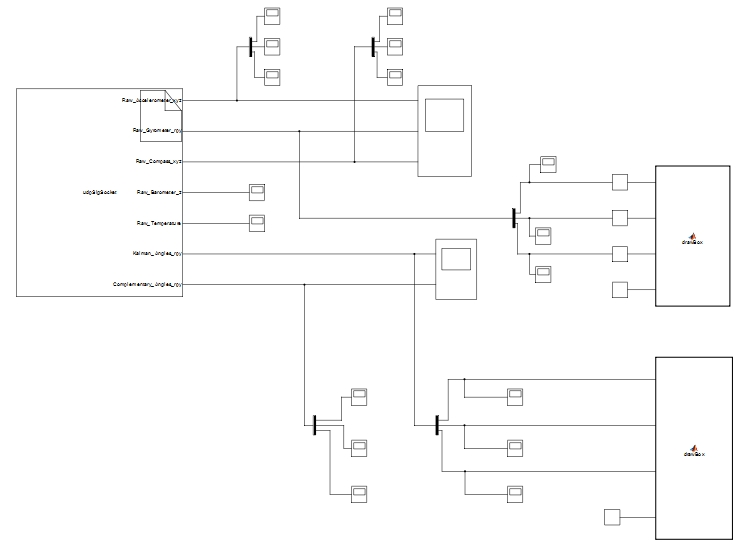
\includegraphics[width=1\textwidth]{fig/Model}
	\caption{Matlab model}
	\label{fig:model}
\end{figure}

\newpage
With the help of the scopes within this model, the logged data is stored in the Matlab workspace and then it is analyzed with a Matlab file. With the help of this file, a histogram from every sensor is generated. Also the meanvalue and the variance from those sensor is calculated. Finally a plot from the complementary filter and Kalman filter is generated. Also the needed minmum and maximum values of the magnetic sensor is stored. This needs to be done to reduce the influences of hard magnetic parts to the magnetic sensor. Those stored minmium and maximum values are then written in a header file (OrientationDefines.h) which needs to be copied to the folder of the Orientation.c and Orientation.h files. To achieve the best performance, the description of chapter \ref{chap:angle} needs to be followed.

\lstset{language=Matlab,%
backgroundcolor=\color{white}  
}

\begin{lstlisting}
headerFileName = 'OrientationDefines.h';

%Acceleration sensor
figure(1)
%plot histogram of ax and calculate meanvalue and variance
subplot(3,1,1)
hist(ax.signals.values(:),50);
    M=mean(ax.signals.values(:));
    V=var(ax.signals.values(:));
title('Acceleration sensor')
disp(['Meanvalue: ' num2str(M)])
xlabel({'Raw data of sensor ax' ['Mean: ' num2str(M)] ['Varianz: ' num2str(V)]}) % x-axis label

%plot histogram of ay and calculate meanvalue and variance
subplot(3,1,2)
hist(ay.signals.values(:),50);
    M=mean(ay.signals.values(:));
    V=var(ay.signals.values(:));
xlabel({'Raw data of sensor ay' ['Mean: ' num2str(M)] ['Varianz: ' num2str(V)]}) % x-axis label
ylabel('Count of appearance') % y-axis label

%plot histogram of az and calculate meanvalue and variance
subplot(3,1,3)
hist(az.signals.values(:),50);
    M=mean(az.signals.values(:));
    V=var(az.signals.values(:));
xlabel({'Raw data of sensor az' ['Mean: ' num2str(M)] ['Varianz: ' num2str(V)]}) % x-axis label

%Magnetic sensor
figure(2)
%plot histogram of mx and calculate meanvalue and variance
subplot(3,1,1)
hist(mx.signals.values(:),50);
    M=mean(mx.signals.values(:));
    V=var(mx.signals.values(:));
title('Magnetic sensor')
disp(['Meanvalue: ' num2str(M)])
xlabel({'Raw data of sensor mx' ['Mean: ' num2str(M)] ['Varianz: ' num2str(V)]}) % x-axis label

%plot histogram of my and calculate meanvalue and variance
subplot(3,1,2)
hist(my.signals.values(:),50);
    M=mean(my.signals.values(:));
    V=var(my.signals.values(:));
xlabel({'Raw data of sensor my' ['Meanvalue: ' num2str(M)] ['Varianz: ' num2str(V)]}) % x-axis label
ylabel('Count of appearance') % y-axis label

%plot histogram of mz and calculate meanvalue and variance
subplot(3,1,3)
hist(mz.signals.values(:),50);
    M=mean(mz.signals.values(:));
    V=var(mz.signals.values(:));
xlabel({'Raw data of sensor mz' ['Meanvalue: ' num2str(M)] ['Variance: ' num2str(V)]}) % x-axis label

%Gyroscope sensor
figure(3)
%plot histogram of pitch and calculate meanvalue and variance
subplot(3,1,1)
hist(pitch.signals.values(:),50);
    M=mean(pitch.signals.values(:));
    V=var(pitch.signals.values(:));
title('Gyroscope sensor')
disp(['Meanvalue: ' num2str(M)])
xlabel({'Raw data of sensor pitch rate' ['Mean: ' num2str(M)] ['Varianz: ' num2str(V)]}) % x-axis label

%plot histogram of roll and calculate meanvalue and variance
subplot(3,1,2)
hist(roll.signals.values(:),50);
    M=mean(roll.signals.values(:));
    V=var(roll.signals.values(:));
xlabel({'Raw data of sensor roll rate' ['Meanvalue: ' num2str(M)] ['Varianz: ' num2str(V)]}) % x-axis label
ylabel('Count of appearance') % y-axis label

%plot histogram of yaw and calculate meanvalue and variance
subplot(3,1,3)
hist(yaw.signals.values(:),50);
    M=mean(yaw.signals.values(:));
    V=var(yaw.signals.values(:));
xlabel({'Raw data of sensor yaw rate' ['Meanvalue: ' num2str(M)] ['Variance: ' num2str(V)]}) % x-axis label


%Complementary filter
figure(4)
subplot(3,1,1)
plot(Comp_pitch.time,Comp_pitch.signals.values(:));
title('Complementary filter')
xlabel('time [s]') % x-axis label
ylabel('pitch [degree]') % y-axis label

subplot(3,1,2)
plot(Comp_roll.time,Comp_roll.signals.values(:));
xlabel('time [s]') % x-axis label
ylabel('roll [degree]') % y-axis label

subplot(3,1,3)
plot(Comp_yaw.time,Comp_yaw.signals.values(:));
xlabel('time [s]') % x-axis label
ylabel('yaw [degree]') % y-axis label


%Kalman filter
figure(5)
subplot(3,1,1)
plot(Kalman_pitch.time,Kalman_pitch.signals.values(:));
title('Kalman filter')
xlabel('time [s]') % x-axis label
ylabel('pitch [degree]') % y-axis label

subplot(3,1,2)
plot(Kalman_roll.time,Kalman_roll.signals.values(:));
xlabel('time [s]') % x-axis label
ylabel('roll [degree]') % y-axis label

subplot(3,1,3)
plot(Kalman_yaw.time,Kalman_yaw.signals.values(:));
xlabel('time [s]') % x-axis label
ylabel('yaw [degree]') % y-axis label

%min max of magnetic sensor
maxz=max(mz.signals.values)*1000000;
minz=min(mz.signals.values)*1000000;
maxy=max(my.signals.values)*1000000;
miny=min(my.signals.values)*1000000;
maxx=max(mx.signals.values)*1000000;
minx=min(mx.signals.values)*1000000;

fprintf('\n');
disp('Calibration Data:');
disp('=================');
disp(['Min_X: ' num2str(minx)])
disp(['Max_X: ' num2str(maxx)])
disp(['Min_Y: ' num2str(miny)])
disp(['Max_Y: ' num2str(maxy)])
disp(['Min_Z: ' num2str(minz)])
disp(['Max_Z: ' num2str(maxz)])
fprintf('\n');

disp('==================================');
disp('Generating Calibration-Header-File');
disp('==================================');

disp(['Writing header ', headerFileName, ' ...' ]);
fileID = fopen(headerFileName,'w');
fprintf(fileID,'/*!\n');
fprintf(fileID,' * \\file OrientationDefines.h\n');
fprintf(fileID,' */\n');
fprintf(fileID,'\n');
fprintf(fileID,'#ifndef SIG_ORIENTATION_ORIENTATIONDEFINES_H_\n');
fprintf(fileID,'#define SIG_ORIENTATION_ORIENTATIONDEFINES_H_\n');
fprintf(fileID,'\n');
fprintf(fileID,'//Defines for Acceleration Magnetic angle calculation (automatic calibration via MATLAB)\n');
fprintf(fileID,'#define M_SIGORI_MAG_MINX_F64	%.9f\n',minx);
fprintf(fileID,'#define M_SIGORI_MAG_MAXX_F64	%.9f\n',maxx);
fprintf(fileID,'#define M_SIGORI_MAG_MINY_F64	%.9f\n',miny);
fprintf(fileID,'#define M_SIGORI_MAG_MAXY_F64	%.9f\n',maxy);
fprintf(fileID,'#define M_SIGORI_MAG_MINZ_F64	%.9f\n',minz);
fprintf(fileID,'#define M_SIGORI_MAG_MAXZ_F64	%.9f\n',maxz);
fprintf(fileID,'\n');
fprintf(fileID,'#endif /* SIG_ORIENTATION_ORIENTATIONDEFINES_H_ */\n');
fclose(fileID);
disp('Done');
fprintf('\n');
disp('Calibration successfully processed.');

\end{lstlisting}
\chapter{Angle calculation}
\label{chap:angle}

\section{Calculation of the orientation angles}
\label{sec:CalcAngle}
The Kalman filter and the complementary filter need both angles as input. Those angles are calculated with the acceleration sensor and with the gyroscope. The gyroscope sensor is used as main input and is corrected by the acceleration/magnetic sensor. The reason why both are used is already described in the Sensor fusion chapter.\\
To achieve an angle from the gyroscope, the values from the sensor needs to be integrated. The following formulas show the integration part of the function of the gyroscope which runs on the Raspberry Pi. It is located in the folder 'sig/Orientientation/' in the file Orientation.c in the function 'm\_sigOri\_calcGyroAnglePerStep\_st()'. This function calculates the angle which since the last call is made.
\begin{align}
roll_{angle}&=roll_{rate}*deltaT\\
pitch_{angle}&=pitch_{rate}*deltaT\\
yaw_{angle}&=yaw_{rate}*deltaT
\end{align}
To make this code independent from any timestep, it calculates locally the time difference 'deltaT' between the last call. To make this possible the 'gettimeofday' function is used. Because of that any jitter will not make a problem. Also the gyroscope sensor gets automatically offset corrected when the code is started.\\\\
To get an angle from the acceleration/magnetic sensor the following calculation is needed. It is located in the function 'm\_sigOri\_calcAccMagAngle\_st()' in the same file like mentioned before.\\
First the roll angle is calculated:
\begin{align}
roll_{angle\_rad}&=atan2\left(\frac{acc_{y\_axis}}{acc_{z\_axis}}\right)\\
		roll_{angle\_deg}&=-roll_{angle\_rad}*180/Pi
\end{align}

Then the pitch is calculated:
\begin{align}
pitch_{angle\_rad}&=atan\left(-\frac{acc_{x\_axis}}{acc_{y\_axis}*sin(roll_{angle\_rad})+acc_{z\_axis}*cos(roll_{angle\_rad})}\right)\\
pitch_{angle\_deg}&=-pitch_{angle\_rad}*180/Pi
\end{align}

Last step is the calculation of the yaw angle. The yaw angle can not be calculated by the acceleration sensor, only the magnetic sensor can be used for this. But the magnetic sensor can not directly be used. Additional a magnetic tilt compensation needs to be done. The following formulas show the calculation steps.\\
\begin{align}
divider=mag_{x\_axis}&*cos(pitch_{angle\_rad})+\\
mag_{y\_axis}&*sin(pitch_{angle\_rad})*sin(roll_{angle\_rad})+\\
mag_{z\_axis}&*sin(pitch_{angle\_rad})*cos(roll_{angle\_rad})
\end{align}
\begin{align}		
yaw_{angle\_rad}&=atan2\left(\frac{mag_{z\_axis}*sin(roll_{angle\_rad})-mag_{y\_axis}*cos(roll_{angle\_rad})}{divider}\right)\\
yaw_{angle\_deg}&=yaw_{angle\_rad}*180/Pi
\end{align}
With this, the implementation of the fusion filter were done and proved. First the results seem to be correct like can be seen in figure \ref{fig:initial_angle}.

\begin{figure}[H]
	\centering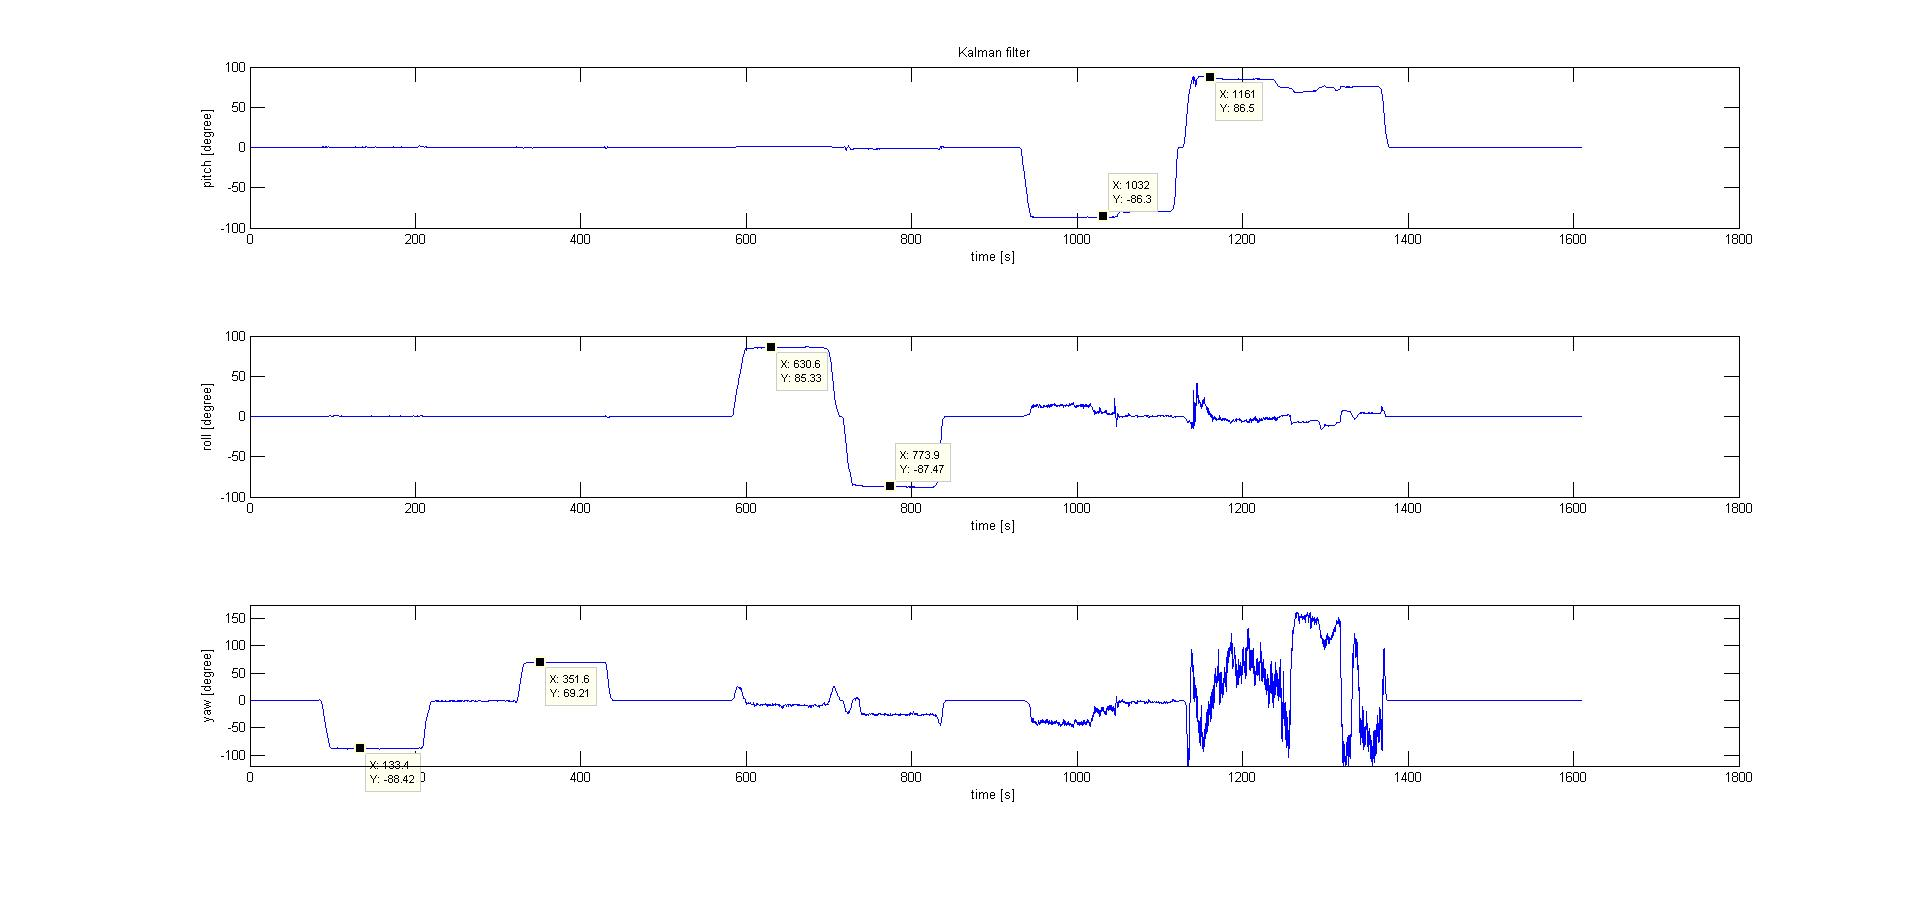
\includegraphics[width=1.0\textwidth]{fig/initial_Kalman}
	\caption{First result Kalman filter}
	\label{fig:initial_angle}
\end{figure}
\section{Magnetic sensor test}
\label{sec:MagSensTest}
As can be seen there is a problem with the yaw angle when a pitch angle is applied. This is no solution which can be used in the quadrocopter. So additional tests are made. After some time the problem was detected. Because just the yaw angle makes some problem, the main observation layed on the magnetic sensor. Figure \ref{fig:field_weak} shows the measured magnetic field.
\begin{figure}[H]
	\centering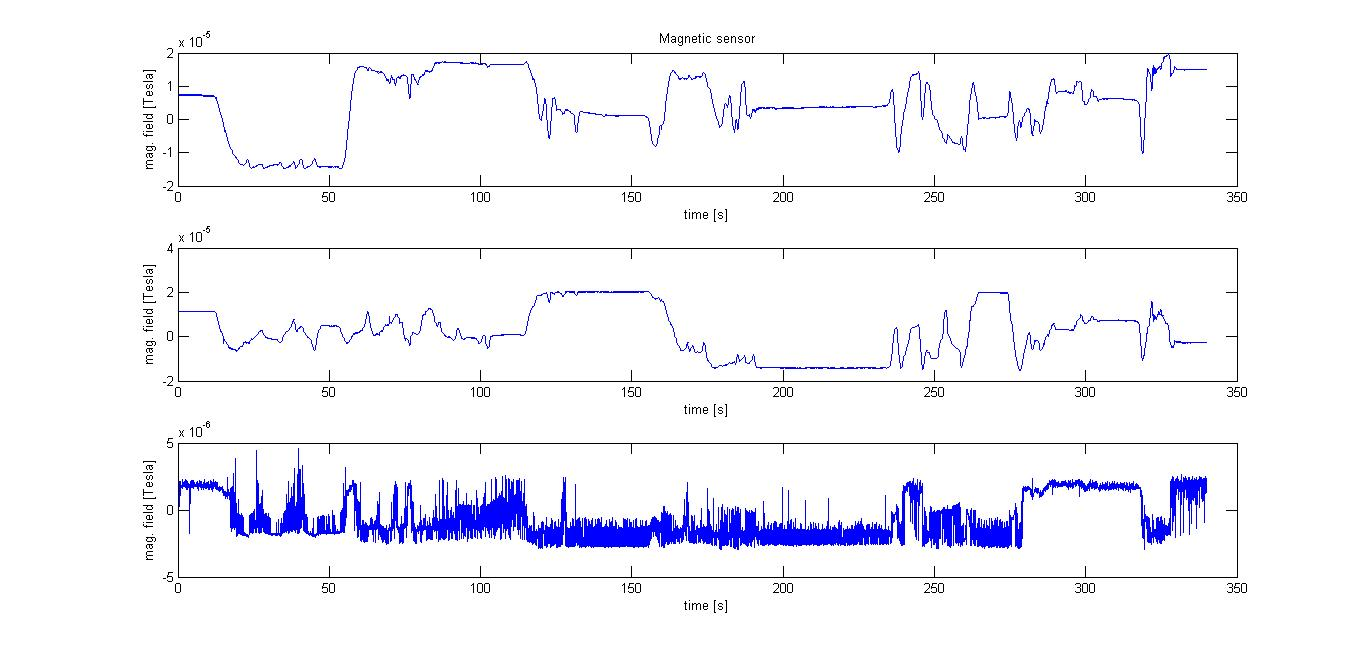
\includegraphics[width=1.0\textwidth]{fig/field_weak}
	\caption{Weak magnetic field strength}
	\label{fig:field_weak}
\end{figure}
The problem can directly be seen. The measured field strength should be nearly the same on all axis. The field strength on the x-axis and y-axis is the same. The z-axis delivers only just one tenth of the normal value. Because of that the noise on the sensor is in the same height like the signal and therefor aquiring not possible. First the position of the mounted IMU is disputed.
After changing the following sensor values of the magnetic sensor can be achieved.
\begin{figure}[H]
	\centering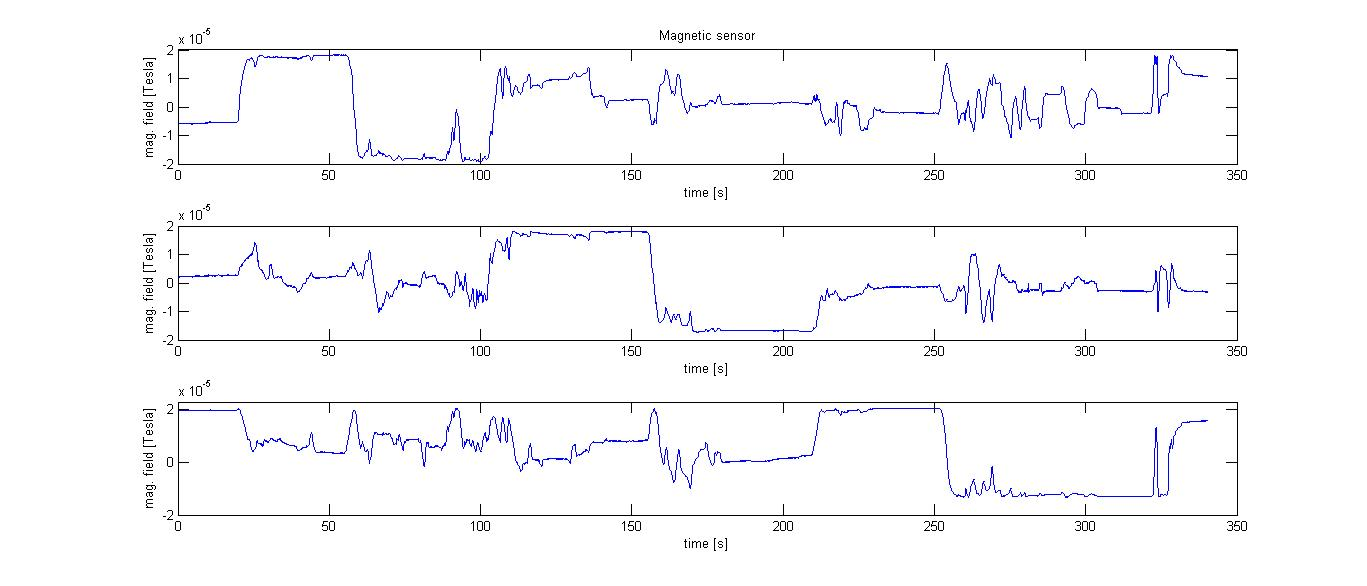
\includegraphics[width=1.0\textwidth]{fig/field_strong}
	\caption{Strong magnetic field strength}
	\label{fig:field_strong}
\end{figure}
By comparing the measurement of the initial positioning of the IMU with the new one, the strength on the z-axis is significantly higher. Also the strength on the three axis are nearly the same. So for further usage the new position is used. 

\section{Improvement magnetic sensor}
\label{sec:ImpMagSens}
The figures \ref{fig:pos_neu1} and \ref{fig:pos_neu2} shows the comparison of the mounting.
\begin{figure}[H]
	\centering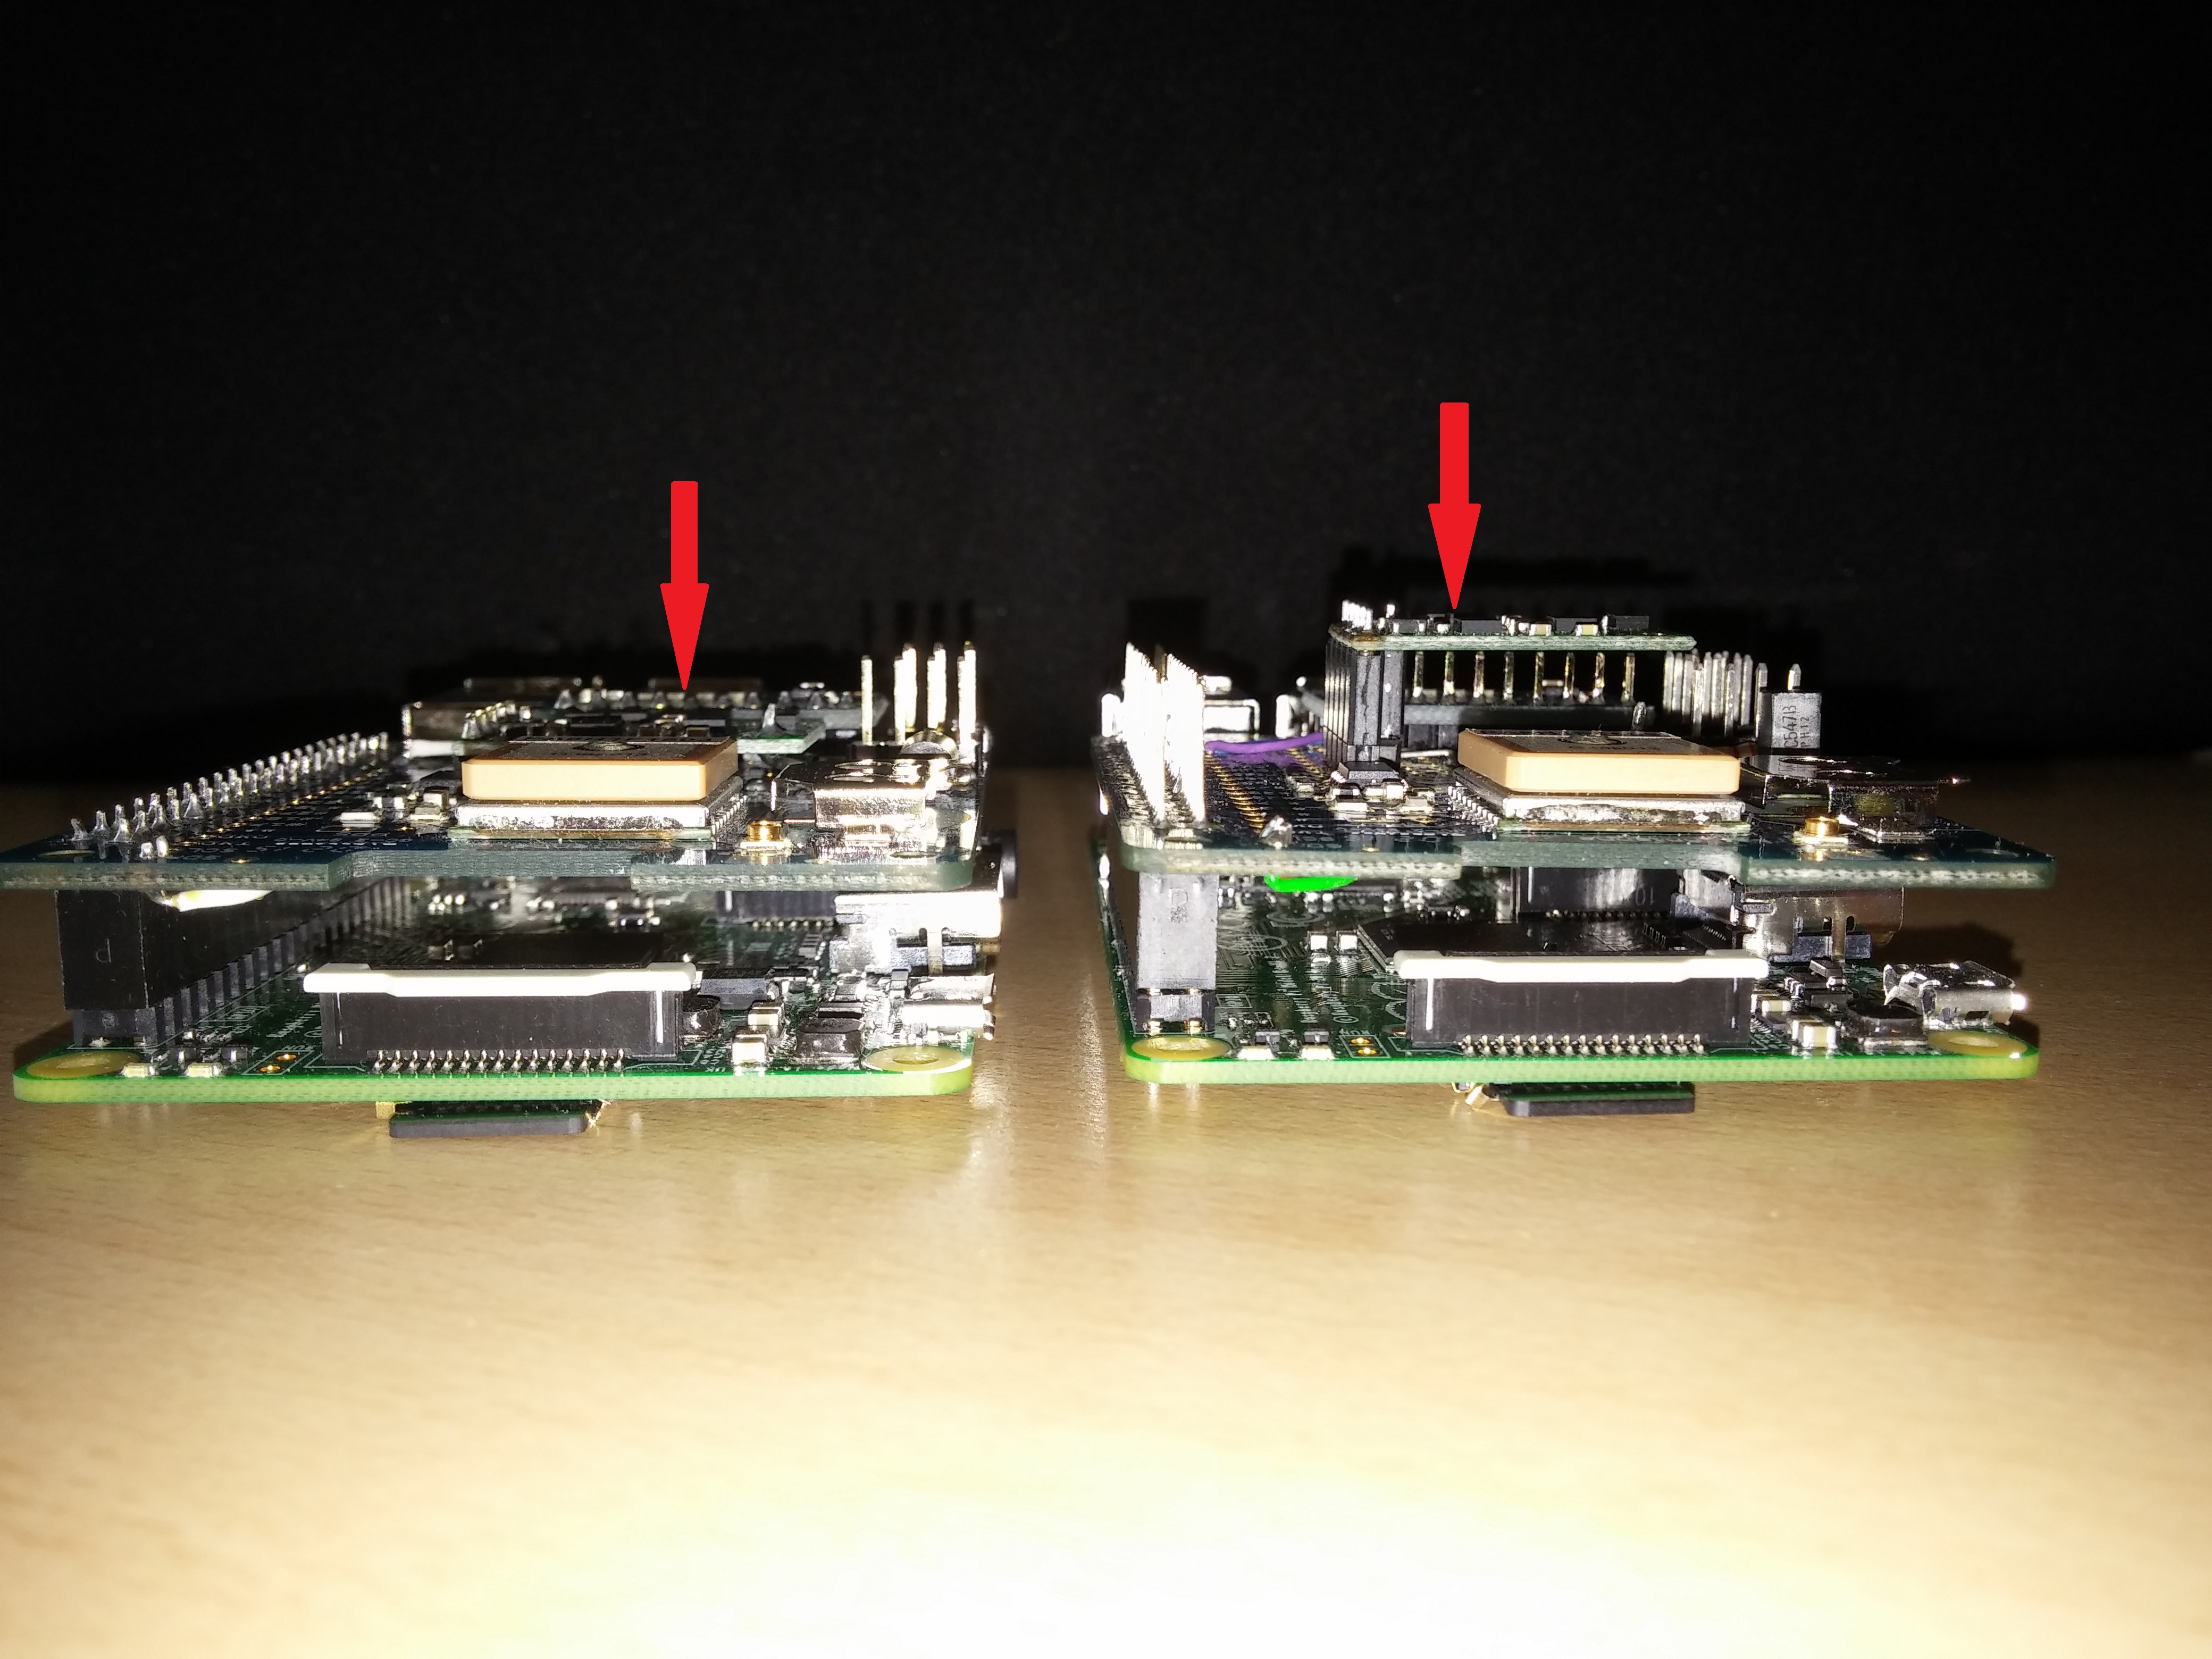
\includegraphics[width=0.6\textwidth]{fig/pos_neu1}
	\caption{New positioning of IMU 1}
	\label{fig:pos_neu1}
\end{figure}
\begin{figure}[H]
	\centering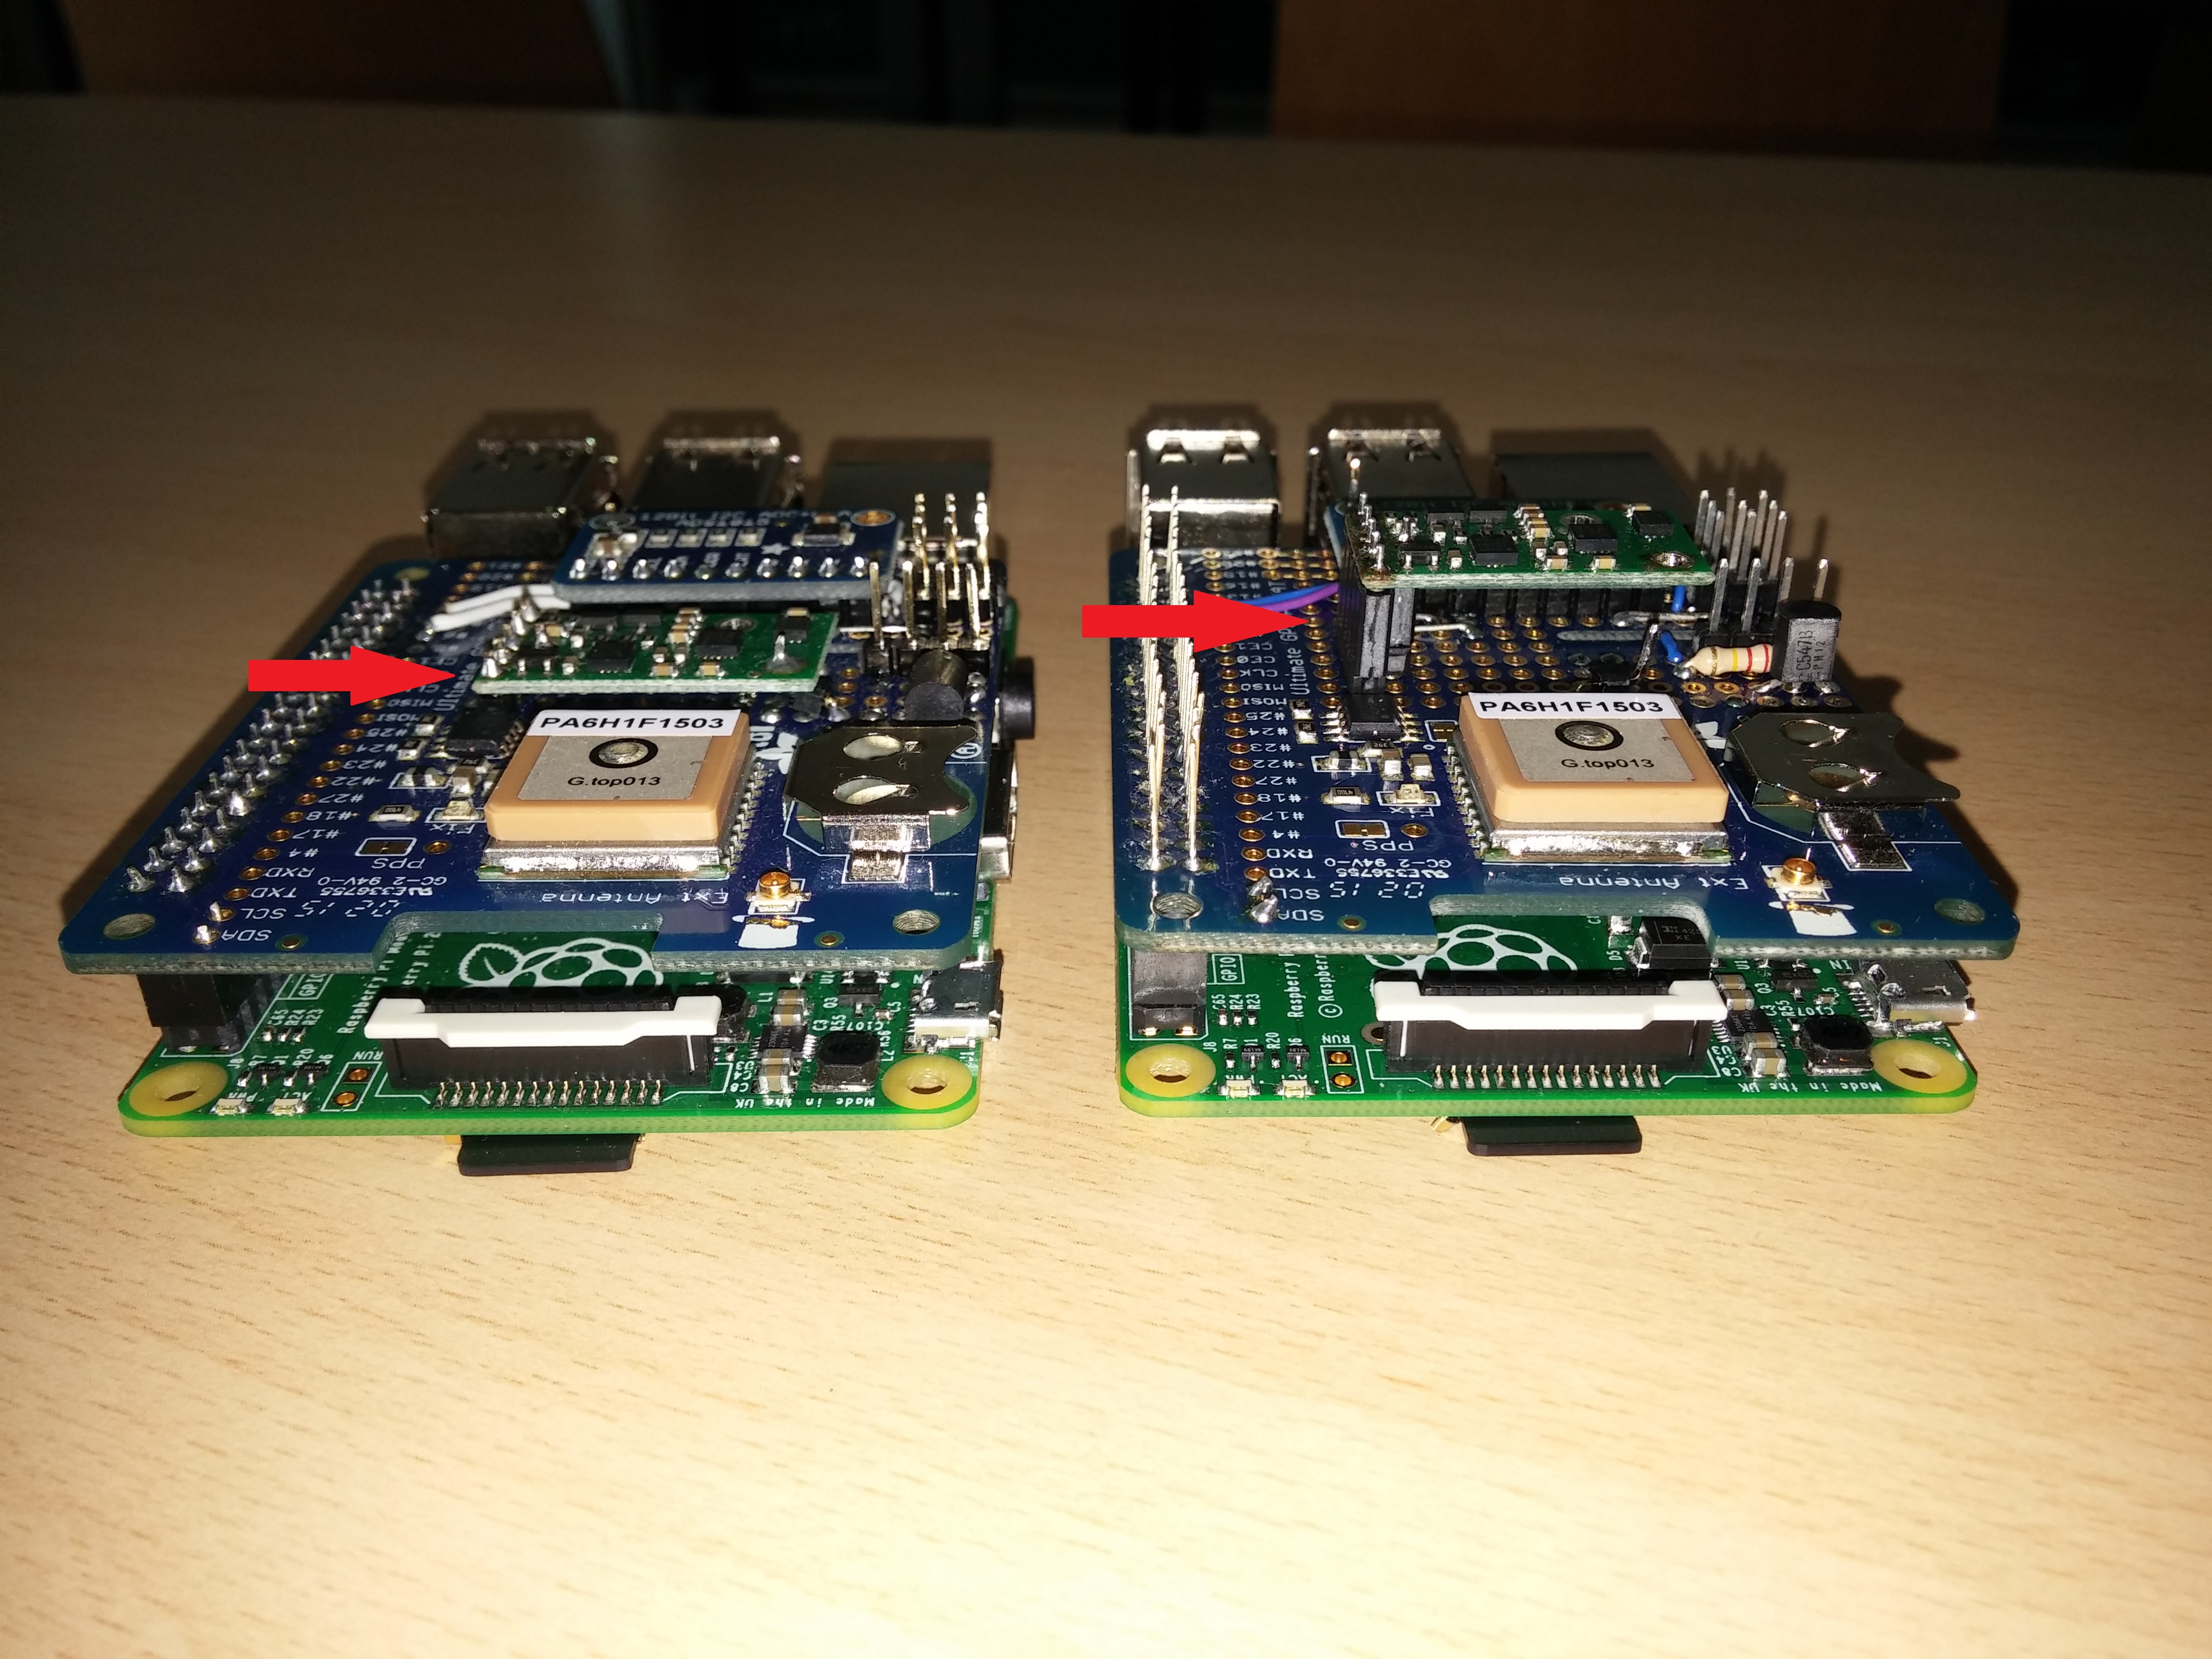
\includegraphics[width=0.6\textwidth]{fig/pos_neu2}
	\caption{New positioning of IMU 2}
	\label{fig:pos_neu2}
\end{figure}
The left PCB shows the old position and the right the new position. As can be seen just the height of the mounted IMU has to be changed. Due to the tests a distance of approximately 1cm seems to be enough. So the wiring can be kept as it is.\\
Additionally to reduce the really high influences of near metallic parts, a hard magnetic offset compensation needs to be done. Also a scaling is done. The following calculations which run in the function 'm\_sigOri\_calcAccMagAngle\_st()' are done within every step.
\begin{align}
mag_{x\_axis}=(mag_{x\_axis}-logged_{min\_x})/(logged_{max\_x}-logged_{min\_x})*2-1\\
mag_{y\_axis}=(mag_{y\_axis}-logged_{min\_y})/(logged_{min\_y}-logged_{min\_y})*2-1\\
mag_{z\_axis}=(mag_{z\_axis}-logged_{min\_z})/(logged_{min\_z}-logged_{min\_z})*2-1
\end{align}
To achieve the full range of the all three sensors the scope of Matlab can be used. The m-file which is mentioned before creates directly the header-file for the code. The improved results due to the changes which are made here can be seen in the second output of the Kalman filter and complementary filter in chapter \ref{chap:ComplementaryFilter} and \ref{chap:KalmanFilter}.
\chapter{Complementary-Filter}
\label{chap:ComplementaryFilter}

The first approach for a sensor fusion is the complementary filter. This filter uses a highpass filter for the gyroscopes and a lowpass filter for the acceleration sensor. The highpass filter is used after the integration of the rotation rates. This can be seen in figure \ref{fig:complementary}.\\
\begin{figure}[H]
	\centering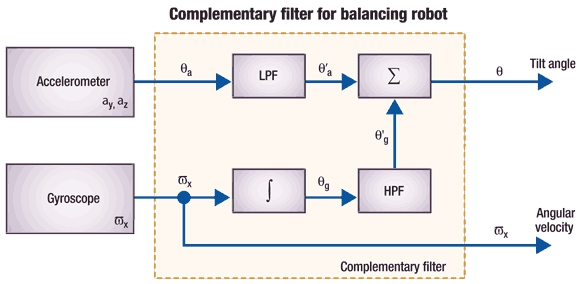
\includegraphics[width=1\textwidth]{fig/Complementary.jpg}
	\caption{Complementary-Filter\cite{doc:STM}}
	\label{fig:complementary}
\end{figure}
The implementation effort is extremely lower than with the Kalman Filter. Because here not matrices and matrix operations are needed. Also are there less calculations and so fits this algorithm better to microprocessors. The only thing what needs to be checked is the lowpass/highpass-filter coefficient. Next the needed calculations are mentioned to show the difference of the complementary and Kalman filter.
\begin{itemize}
	\item Calculation of the accelerometer and magnetometer angles
	\item Calculation of the gyroscope angles
	\item Complementary-Filter usage with defined filter time of the lowpass and highpass-filter
\end{itemize}
\chapter{Kalman-Filter}
\label{chap:KalmanFilter}

For the Kalman filter the noise of the measurement and the process has to be set up. This noise values are the variances of the used sensors and of the process. In the calculation process are those matrices named $\underline Q$ and $\underline R$. The matrix $\underline Q$ uses the variances of the process noise and the matrix $\underline R$ uses the variances of the noise of the sensors.\\\\
\underline{Prediction step:}\\\\
Predict the next state:
\begin{align}
\vec x_k = \underline{A}\vec x_{k-1}+\underline{B}\vec u_{k-1}
\label{equ:Kalman1}
\end{align}
Predict the covariance for the next step:
\begin{align}
\underline{P}_k = \underline{A}\underline{P}_{k-1}\underline{A}^T+\underline{Q}
\label{equ:Kalman2}
\end{align}
\underline{Correction step:}\\\\
Computation of the Kalman gain:
\begin{align}
\underline{K}_k = \underline{P}_k	\underline{H}^T(\underline{H}\underline{P}_k\underline{H}^T+\underline{R})^{-1}
\label{equ:Kalman3}
\end{align}
Updating state prediction with new measurement:
\begin{align}
\vec x_k = 	\vec x_k+\underline{K}_k(\vec z_k-\underline{H}\vec x_k)
\label{equ:Kalman4}
\end{align}
Updating the error covariance:
\begin{align}
\underline{P}_k = (\underline{I}-\underline{K}_k\underline{H})\underline{P}_k	
\label{equ:Kalman4}
\end{align}
As an initial guess the matrices are set to:
\begin{align}
\underline{Q} &= \begin{pmatrix} 0.005&0&0 \\ 0&0.005&0 \\ 0&0&0.0001 \end{pmatrix}\\
\underline{R} &= \begin{pmatrix} 0.5&0&0 \\ 0&0.5&0 \\ 0&0&0.01 \end{pmatrix}
\end{align}
With those matrices the following result was achieved. To make a test, first the yaw angle is changed in the range of $\pm90 \degree$, after that a roll angle is changed in the range of $\pm90 \degree$ and finally the pitch angle is changed in the range of $\pm90 \degree$. 

\begin{figure}[H]
	\centering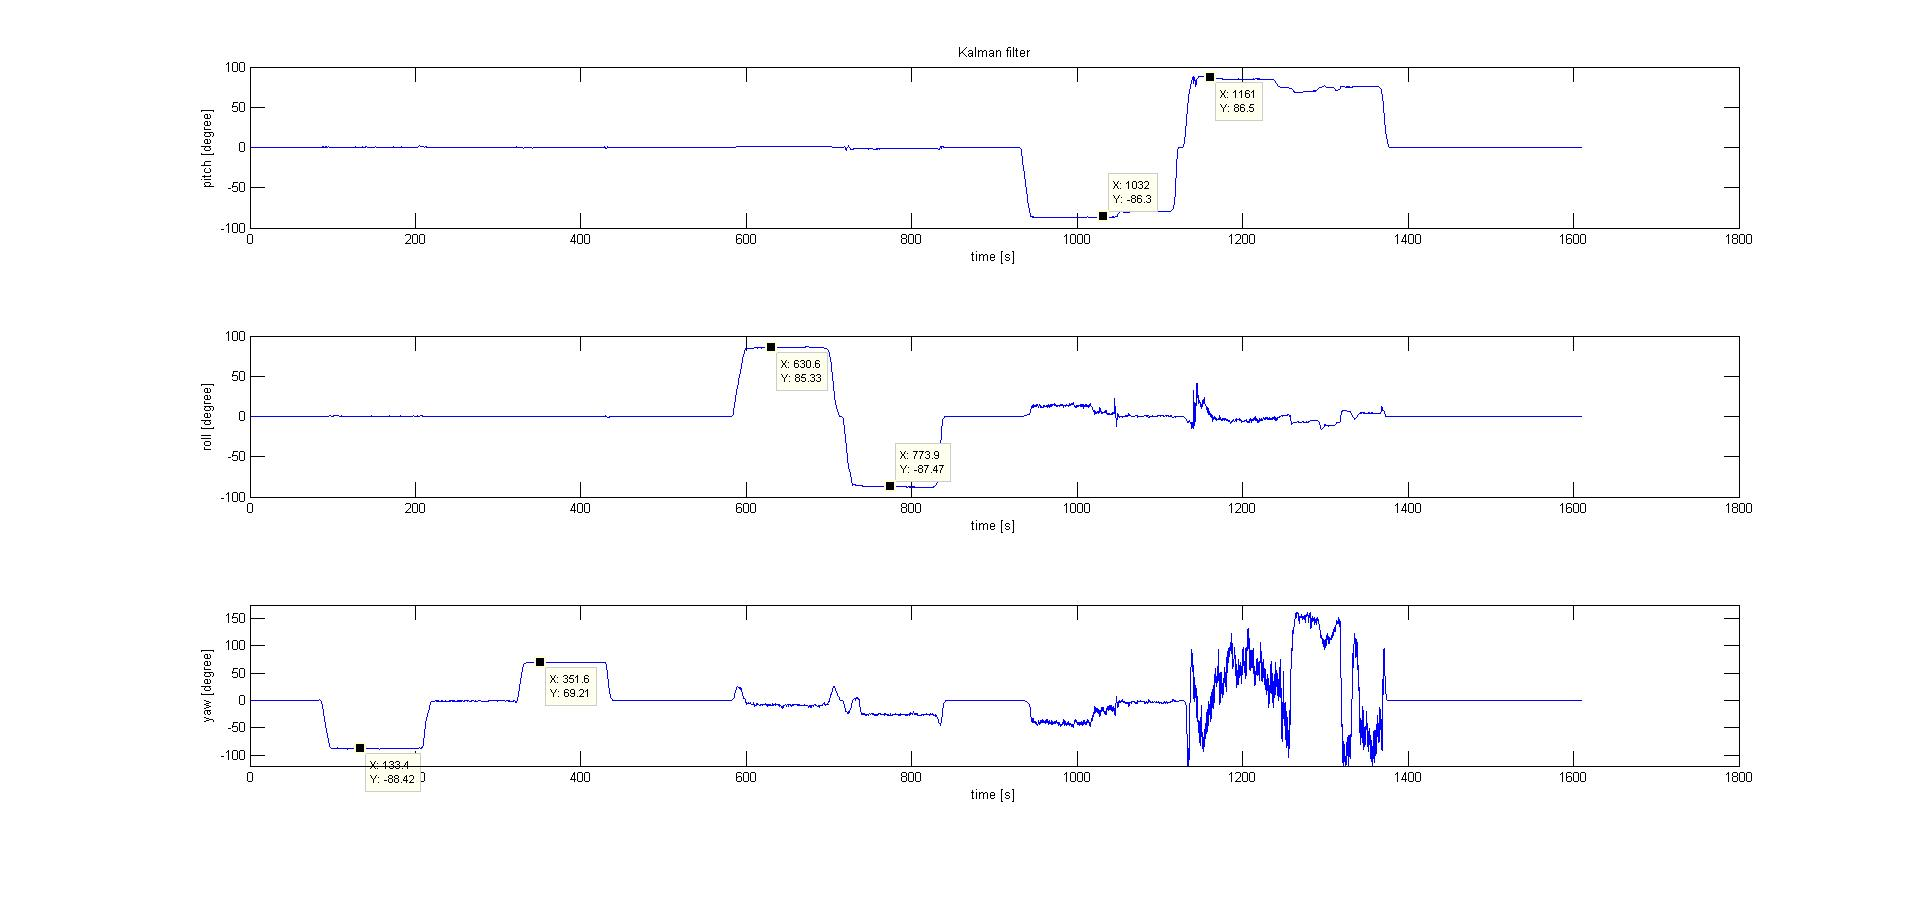
\includegraphics[width=1.0\textwidth]{fig/initial_Kalman}
	\caption{First result Kalman filter}
	\label{fig:initial_Kalman}
\end{figure}

The filter responses in a adequate time. Yaw angle change is like with the complementary filter from -90 degree to just 70 degree. The roll angle changes sufficient. But when changing the pitch angle to high a extreme yaw angle change can be seen. So the next step is to improve the yaw angle, so that it will reach also the +90 degree. Also the yaw change during pitch will be observed. After measuring the meanvalue and variances of all sensors they can be used to improve the Kalman filter. The figures \ref{fig:varAcc}, \ref{fig:varGyro} and \ref{fig:varMag} show the logged data.
\begin{figure}[H]
	\centering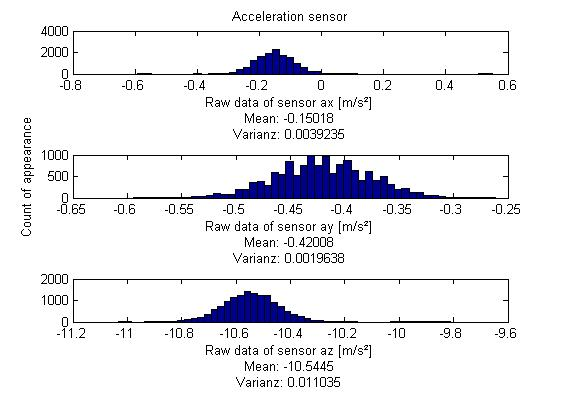
\includegraphics[width=0.8\textwidth]{fig/varAcc3}
	\caption{Analyzing the acceleration sensor}
	\label{fig:varAcc}
\end{figure}
\begin{figure}[H]
	\centering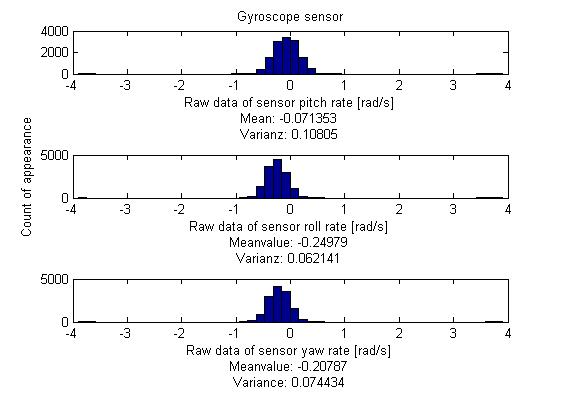
\includegraphics[width=0.8\textwidth]{fig/varGyro3}
	\caption{Analyzing the gyroscope sensor}
	\label{fig:varGyro}
\end{figure}
\begin{figure}[H]
	\centering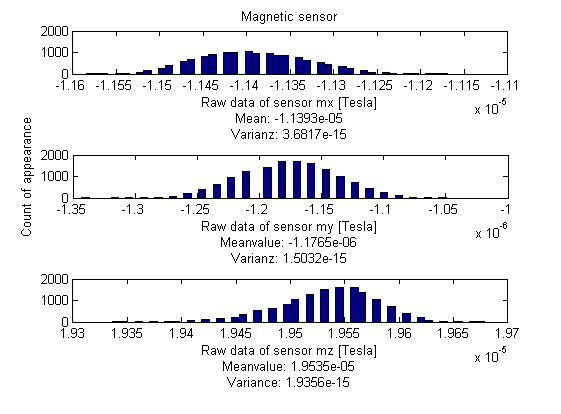
\includegraphics[width=0.8\textwidth]{fig/varMag3}
	\caption{Analyzing the magnetic sensor}
	\label{fig:varMag}
\end{figure}
First the matrix $\underline Q$, the variances of the process noise and the matrix $\underline R$, the variances of the measured sensor noises are changed by using the measured values. The new values are:\\
\begin{align}
\underline{Q} &= \begin{pmatrix} 0.005&0&0 \\ 0&0.005&0 \\ 0&0&0.005 \end{pmatrix}\\
\underline{R} &= \begin{pmatrix} 0.06&0&0 \\ 0&0.1&0 \\ 0&0&0.07 \end{pmatrix}
\end{align}

\begin{figure}[H]
	\centering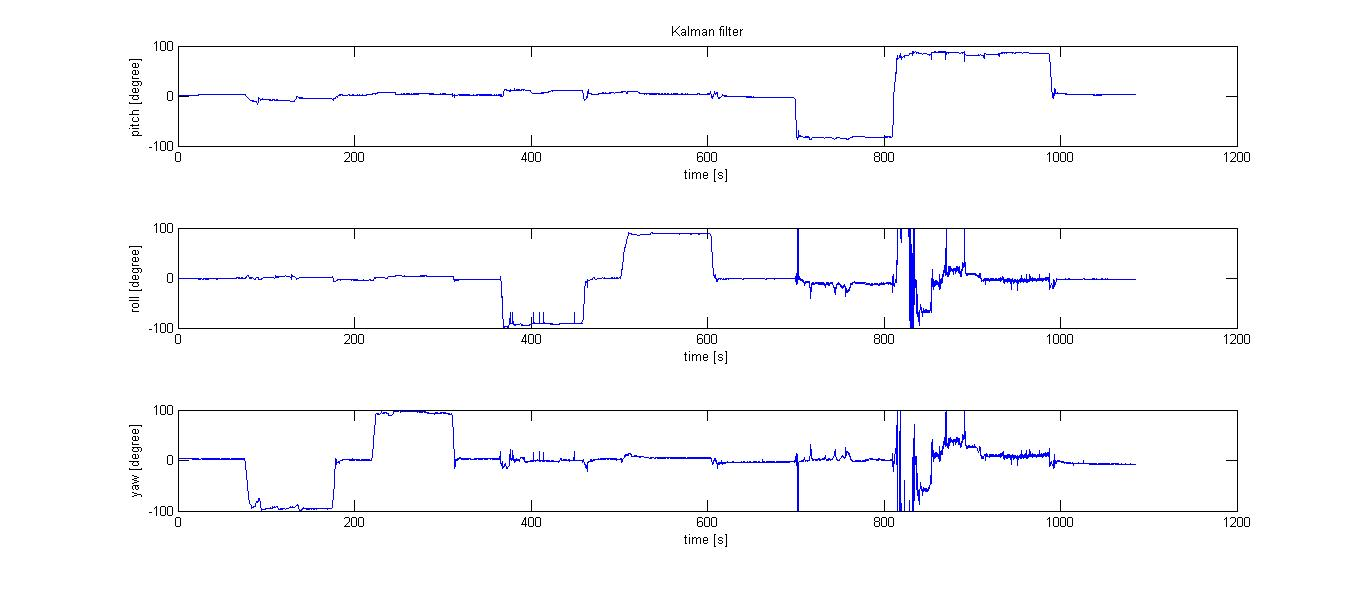
\includegraphics[width=1.0\textwidth]{fig/final_Kalman1}
	\caption{Final result Kalman filter}
	\label{fig:final_Kalman}
\end{figure}
The wanted improving of the yaw angle in reaching the 90 degree when turning 90 degree is succesfully reached. The extreme influences on yaw directly after changing of the rotation angle results from a hand made rotation. The influences on yaw while an other angle is applied is extremely reduced.\\

The last figure shows how off an angle can be when just an gyroscope is used. On the left side the integrated gyroscope can be seen. On the right side, the 3D representation of the fusioned sensors are displayed.
\begin{figure}[H]
	\centering\includegraphics[width=0.6\textwidth]{fig/3D}
	\caption{3D representation of the integrated gyroscope raw values on the left and the fusion filtered on the right}
	\label{fig:3D}
\end{figure}

% % %%%%%% Anhang
\appendix

%\chapter{Kapitel im Anhang}
\label{sec:a-kapitel}

Alles was den Hauptteil unn�tig vergr��ert h�tte, z. B. HW-/SW-Dokumentationen, Bedienungsanleitungen, Code-Listings, Diagramme


% % %%%%%% Literaturverzeichnis (darf im deutschen nicht in den Anhang!)
% Einfaches Literaturverzeichnis
%\begin{thebibliography}{XXXX}
%\bibitem{doc:stz} Thomas Nonnenmacher, LaTeX Grundlagen - Setzen einer wissenschaftlichen Arbeit Skript, 2008,\url{http://www.stz-softwaretechnik.de}; \textit{(Bei STZ Internetseite unter Publikationen - Skripte) [V.\,2.0 26.02.08]}
%
%\bibitem[Gun04]{doc:gun} Karsten G�nther, LaTeX2 --- Das umfassende Handbuch, Galileo Computing, 2004, \url{http://www.galileocomputing.de/katalog/buecher/titel/gp/titelID-768}; \textit{1. Auflage}
%\end{thebibliography}

% Literaturverzeichnis mit Bibtex
%\bibliography{bib/bib}

% %  Inhalt ENDE %%%%%%%%%%%%%%%%%%%%%%%%%%%%%%%%%%%%%%%%%%%%%%%%%%%%%%%%%%
\end{document}
